\chapter{Nonequilibrium clumped isotope signals in microbial methane}
\label{ch:2}
\chaptermark{Survey of \ce{^{13}CH3D in the environment}}




\begin{abstract}
	\noindent Methane is a key component in the global carbon cycle with a wide range
	of anthropogenic and natural sources. While isotopic compositions of
	methane have traditionally aided source identification, the abundance of
	its multiply-substituted ``clumped'' isotopologues (e.g.,
	\textsuperscript{13}CH\textsubscript{3}D) has recently emerged as
	a proxy for determining methane-formation temperatures. However, the
	impact of biological processes on methane's clumped isotopologue
	signature is poorly constrained. Here, we show that methanogenesis
	proceeding at relatively high rates in cattle, surface environments, and
	laboratory cultures exerts kinetic control on
	\textsuperscript{13}CH\textsubscript{3}D abundances and results in
	anomalously elevated formation temperature estimates. We demonstrate
	quantitatively that H\textsubscript{2} availability accounts for this
	effect. Clumped methane thermometry can therefore provide
	constraints on the generation of methane in diverse settings, including
	continental serpentinization sites and ancient, deep groundwaters.
\end{abstract}

\vspace*{\fill}

\noindent \rule{\textwidth}{0.4pt}\\

{\small
	
	\noindent A version of this chapter has been published as:\\
	
	\noindent Wang, D. T.; Gruen, D. S.; Lollar, B. S.; Hinrichs, K.-U.; Stewart, L. C.; Holden, J. F.; Hristov, A. N.; Pohlman, J. W.; Morrill, P. L.; Könneke, M.; Delwiche, K. B.; Reeves, E. P.; Sutcliffe, C. N.; Ritter, D. J.; Seewald, J. S.; McIntosh, J. C.; Hemond, H. F.; Kubo, M. D.; Cardace, D.; Hoehler, T. M. \& Ono, S. (2015) Nonequilibrium clumped isotope signals in microbial methane. \emph{Science,} \textbf{348}, 428--431.  \href{http://dx.doi.org/10.1126/science.aaa4326}{\nolinkurl{doi: 10.1126/science.aaa4326}}\\
	
	\noindent Copyright © 2015, The Authors.  AAAS maintains exclusive rights to use and authorize use of this article under its License to Publish.  Reproduction in this thesis is permitted under the terms of this agreement.
	
}

\clearpage

\section{Main Text} \label{main-text}
%\addcontentsline{toc}{section}{\protect\numberline{}Main Text}
%\addcontentsline{toc}{section}{Main Text}


\noindent Carbon (\textsuperscript{13}C/\textsuperscript{12}C) and hydrogen (D/H)
isotope ratios of methane are widely applied for distinguishing
microbial from thermogenic methane in the environment \parencite{Baldassare++_2014_AAPGB,Flores++_2008_IJCG,Pohlman++_2009_EPSL,SherwoodLollar++_2008_GCA,SherwoodLollar++_2002_N,Welhan+Lupton_1987_AAPGB,Whiticar_1990_OG} as well as for apportioning pathways of microbial
methane production \parencite{Burke++_1988_N,McCalley++_2014_N,Whiticar++_1986_GCA}. This bulk isotope approach,
however, is largely based on empirical observations, and different
origins of methane often yield overlapping characteristic isotope
signals \parencite{Pohlman++_2009_EPSL,Whiticar_1990_OG,Etiope+SherwoodLollar_2013_RG,Schoell_1988_CG,Whiticar_1999_CG}. Beyond conventional
bulk isotope ratios, it has become possible to precisely measure the
abundance of multiply-substituted ``clumped'' isotopologues (e.g.,
\textsuperscript{13}CH\textsubscript{3}D) \parencite{Ono++_2014_AC,Stolper++_2014_GCA}. In
particular, the abundances of clumped isotopes makes it possible to obtain information
about the temperature at which C--H bonds were formed or last
equilibrated \parencite[][and \autoref{fig:2:S1}]{Ono++_2014_AC}. Formation temperatures
of both thermogenic and microbial methane in natural gas reservoirs can
be estimated on the basis of clumped isotopologues \parencite{Stolper++_2014_S}. The
mechanisms by which isotopologues attain distributions consistent with
thermodynamic equilibrium, however, remain unclear because bulk methane
isotopes (δ\textsuperscript{13}C and δD) often reflect kinetic isotope
fractionations \parencite{Whiticar_1999_CG,Valentine++_2004_GCA}, and H-isotope exchange between
methane and water is sluggish \parencite{Reeves++_2012_GCA}.

To test if clumped methane thermometry can be widely applied for methane
sources beyond natural gas reservoirs, we examined methane samples from
diverse systems, including lakes, wetlands, cow rumen, laboratory
cultures of methanogenic microbes, and geological settings that may
support abiogenic methane production. We measured the relative abundances of four methane
isotopologues (\textsuperscript{12}CH\textsubscript{4},
\textsuperscript{13}CH\textsubscript{4},
\textsuperscript{12}CH\textsubscript{3}D and
\textsuperscript{13}CH\textsubscript{3}D) using a recently-developed
tunable laser spectroscopy technique \parencite[][and \autoref{materials-and-methods}]{Ono++_2014_AC}.


\begin{SCfigure*}[][htbp]
	\centering
	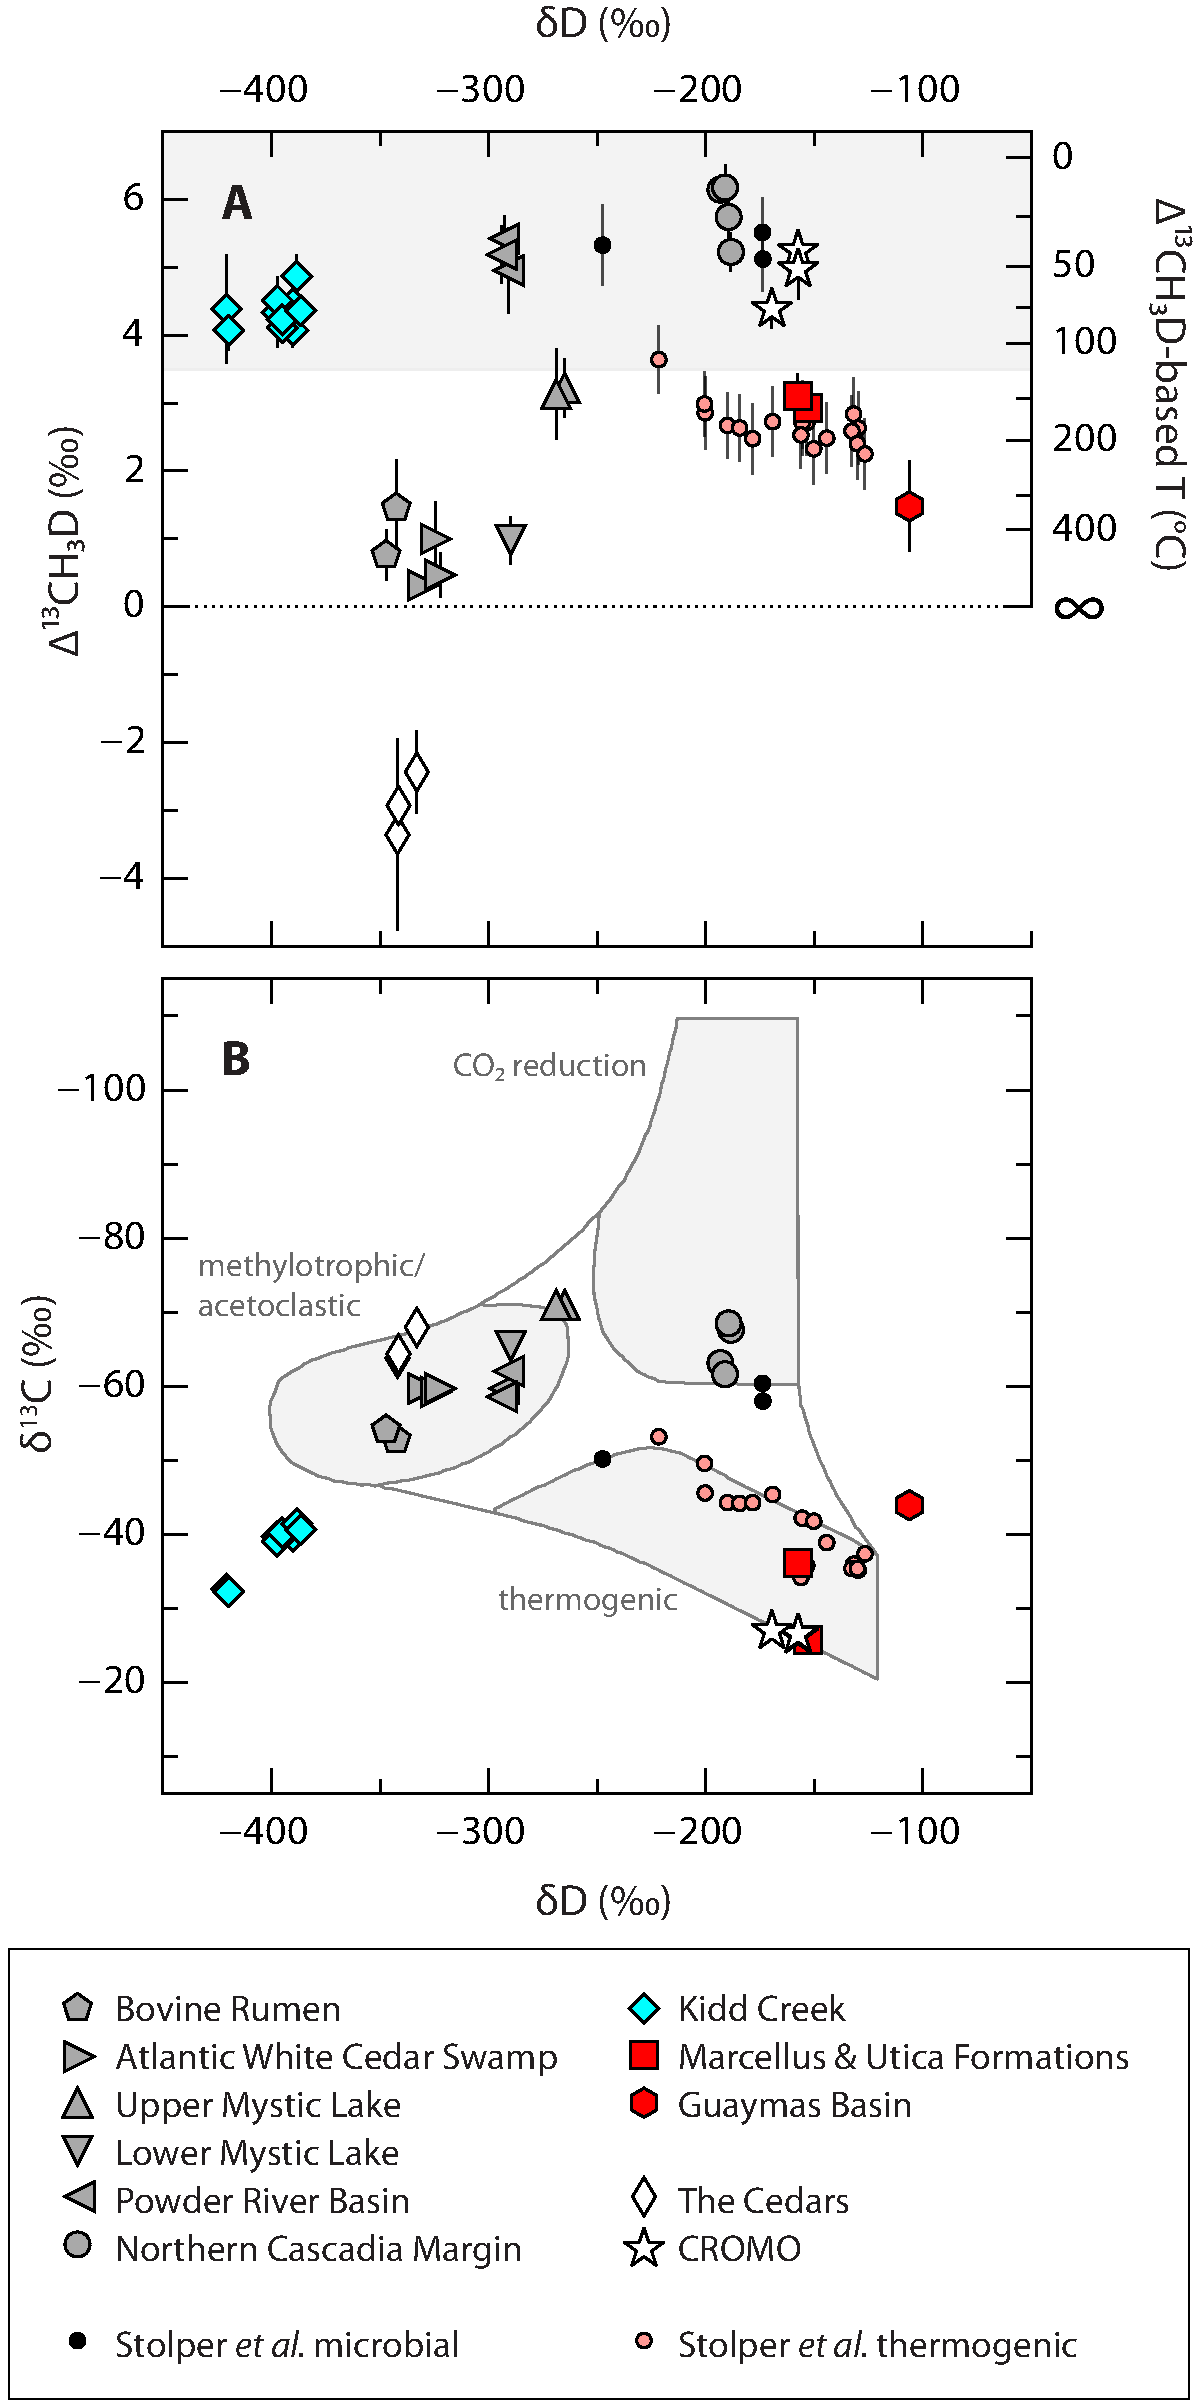
\includegraphics[width=0.5\linewidth]{figures/Fig2.1}
	\caption[Isotopologue compositions of methane samples from an environmental survey]{Isotopologue compositions of methane samples. \textbf{(A)}
	Δ\textsuperscript{13}CH\textsubscript{3}D plotted against δD. The
	Δ\textsuperscript{13}CH\textsubscript{3}D temperature scale corresponds
	to calibration in \autoref{fig:2:S1}. Error bars are 95\% confidence intervals
	(\autoref{tab:2:S1}). Data from \textcite{Stolper++_2014_S} were scaled to their
	corresponding Δ\textsuperscript{13}CH\textsubscript{3}D values
	\parencite{Stolper++_2014_GCA}. The shaded area represents the temperature range within
	which microbial life has been demonstrated to date \parencite{Takai++_2008_PNAS}. The
	hatched line represents Δ\textsuperscript{13}CH\textsubscript{3}D = 0‰ (\textit{T} → $\infty$); data plotting below this line cannot yield corresponding
	apparent temperatures. \textbf{(B)} δ\textsuperscript{13}C plotted
	against δD, showing characteristic fields for different methane sources
	from \textcite{Whiticar_1999_CG}.}
	\label{fig:2:1}
\end{SCfigure*}


Our measurements for dominantly-thermogenic gases from the Marcellus and
Utica Shales \parencite{Baldassare++_2014_AAPGB,Burruss+Laughrey_2010_OG} yielded
Δ\textsuperscript{13}CH\textsubscript{3}D-based temperatures of $147^{+25}_{-22}$\,°C and $160^{+29}_{-25}$\,°C, respectively. The clumped-isotope temperature for the Marcellus
Shale sample is comparable to, although slightly lower than, estimates
by \textcite{Stolper++_2014_S} of 179--207~°C (\autoref{fig:2:1}). In addition,
microbial methane in pore waters and gas hydrates from northern Cascadia
margin sediments \parencite{Pohlman++_2009_EPSL}, and from wells producing from coal seams in
the Powder River Basin \parencite{Flores++_2008_IJCG,Bates++_2011_CG} yielded
Δ\textsuperscript{13}CH\textsubscript{3}D temperatures of 12--42~°C and
35--52~°C, respectively. These are consistent with their expected low
formation temperatures. Furthermore, thermogenic methane sampled from a
hydrothermal vent in the Guaymas Basin, Gulf of California \parencite{Welhan+Lupton_1987_AAPGB},
yielded a Δ\textsuperscript{13}CH\textsubscript{3}D temperature of $326^{+170}_{-95}$\,°C,
within error of the measured vent temperature \parencite[299~°C;][]{Reeves++_2014_PNAS}.
Therefore, our data provide independent support of the hypothesis that
\textsuperscript{13}CH\textsubscript{3}D abundance reflects the
temperature at which methane is generated in these sedimentary basins
\parencite{Stolper++_2014_S}.

In contrast, we found that methane sampled from lakes, a swamp, and the
rumen of a cow carry \textsuperscript{13}CH\textsubscript{3}D signals
that correspond to anomalously high
Δ\textsuperscript{13}CH\textsubscript{3}D temperatures (139--775~°C,
\mrefs[A]{Fig.}{fig:2:1}) that are well above the environmental temperatures (\textless{}40~°C). Such signals are clearly not controlled by equilibrium. Notably, a
positive correlation between Δ\textsuperscript{13}CH\textsubscript{3}D
and the extent of D/H fractionation between methane and environmental
water [$\varepsilon$\textsubscript{methane/water};\footnote{\label{fn:2:epsilon}The abundance of \textsuperscript{13}CH\textsubscript{3}D is
	captured by a metric, Δ\textsuperscript{13}CH\textsubscript{3}D, which
	quantifies its deviation from a random distribution of isotopic
	substitutions amongst all isotopologues in a sample of methane:
	Δ\textsuperscript{13}CH\textsubscript{3}D = ln\,\emph{Q}, where \emph{Q}
	is the reaction quotient of the isotope exchange reaction:
	$ {}^{13}\text{CH}_4+ {}^{12}{\text{CH}}_3\text{D}\rightleftharpoons {}^{13}{\text{CH}}_3\text{D}+ {}^{12}{\text{CH}}_4 $, where the δ-values are
	conventional isotopic notation, e.g., δD =
	(D/H)\textsubscript{sample}/(D/H)\textsubscript{reference} $-$ 1. Mass
	spectrometric measurements yield Δ\textsubscript{18}, a parameter that
	quantifies the combined abundance of
	\textsuperscript{13}CH\textsubscript{3}D and
	\textsuperscript{12}CH\textsubscript{2}D\textsubscript{2}. For most
	natural samples of methane, Δ\textsubscript{18} is expected to be
	directly-relatable to Δ\textsuperscript{13}CH\textsubscript{3}D as
	measured by laser spectroscopy. The D/H fractionation between methane
	and environmental water is defined as $\varepsilon$\textsubscript{methane/water} =
	(D/H)\textsubscript{methane}/(D/H)\textsubscript{water} $-$ 1.} \autoref{fig:2:2}] suggests
a strong link between isotopologue (i.e.,
\textsuperscript{13}CH\textsubscript{3}D) and isotope (D/H)
disequilibria. In contrast, the above mentioned methane samples from
sedimentary basins appear to have attained hydrogen-isotope equilibrium
with associated waters at or near the temperatures indicated by the
Δ\textsuperscript{13}CH\textsubscript{3}D data (\autoref{fig:2:2}).

To confirm these observations from the natural environment, we
demonstrated that strong disequilibrium
\textsuperscript{13}CH\textsubscript{3}D signals are also produced by
cultures of methanogenic archaea in the laboratory (\autoref{fig:2:3}).
Thermophilic methanogens cultured at 40 to 85~°C produced methane with
Δ\textsuperscript{13}CH\textsubscript{3}D values from +0.5 to +2.3‰
(corresponding to Δ\textsuperscript{13}CH\textsubscript{3}D temperatures
of 216--620~°C), and mesophilic methanogens cultured at ambient
temperature produced methane with conspicuously ``anti-clumped''
signatures (i.e., values of Δ\textsuperscript{13}CH\textsubscript{3}D
\textless{} 0‰, for which no apparent temperature can be expressed) as
low as $-$1.3‰ (\autoref{fig:2:3}). Methane from cultures is also characterized by
large kinetic D/H fractionation with respect to water \parencite{Valentine++_2004_GCA,Balabane++_1987_OG}. Because laboratory cultures are grown under optimal
conditions (high H\textsubscript{2} and high CO\textsubscript{2}), these
anti-clumped Δ\textsuperscript{13}CH\textsubscript{3}D and low
$\varepsilon$\textsubscript{methane/water} values are primarily expressions of
kinetic isotope effects. Consequently, the distribution of samples with
Δ\textsuperscript{13}CH\textsubscript{3}D and
$\varepsilon$\textsubscript{methane/water} values in \autoref{fig:2:2} can be explained by
microbial methanogenesis operating on a spectrum between fully kinetic
(low Δ\textsuperscript{13}CH\textsubscript{3}D and low
$\varepsilon$\textsubscript{methane/water}) and equilibrium (high
Δ\textsuperscript{13}CH\textsubscript{3}D and high
$\varepsilon$\textsubscript{methane/water}) end-members.

We constructed a mathematical framework to describe the controls on the
correlation of Δ\textsuperscript{13}CH\textsubscript{3}D and
$\varepsilon$\textsubscript{methane/water} signals from hydrogenotrophic
methanogenesis. The model largely follows those developed for microbial
sulfate reduction \parencite{Rees_1973_GCA,Wing+Halevy_2014_PNAS} and predicts the isotopologue
compositions of product methane as a result of a series of enzymatic
reactions (\autoref{fig:2:S4} and \autoref{model-of-isotopologue-systematics-during-microbial-methanogenesis}). Using isotope fractionation
factors estimated from theory, experiments, and observations as input
parameters (\autoref{tab:2:S3}), our model reproduces the
observed correlation between Δ\textsuperscript{13}CH\textsubscript{3}D
and $\varepsilon$\textsubscript{methane/water} of natural samples (\autoref{fig:2:2}). The
isotopologue compositions of product methane reflect the degree of
metabolic reversibility. Fully reversible reactions yield equilibrium
end-members \parencite{Holler++_2011_PNAS}, while irreversible reactions result in kinetic
(disequilibrium) end-member signals. In this model, the reversibility is
linked to available free energy \parencite{Holler++_2011_PNAS,Wing+Halevy_2014_PNAS}, in this case
expressed as H\textsubscript{2} concentration
({[}H\textsubscript{2}{]}). The model can explain the relationship among
{[}H\textsubscript{2}{]}, $\varepsilon$\textsubscript{methane/water} \parencite{Burke_1993_Chemosphere}, and
Δ\textsuperscript{13}CH\textsubscript{3}D via Michaelis-Menten kinetics,
and can predict the patterns observed in diverse settings ranging from
marine sediments (low {[}H\textsubscript{2}{]}, high
Δ\textsuperscript{13}CH\textsubscript{3}D and
$\varepsilon$\textsubscript{methane/water}) to bovine rumen (high
{[}H\textsubscript{2}{]}, low Δ\textsuperscript{13}CH\textsubscript{3}D
and $\varepsilon$\textsubscript{methane/water}) (\autoref{fig:2:4}). We note that mixing of
methane sources with different δ\textsuperscript{13}C and δD values or
oxidation of methane could also alter the relationships over the primary
signal of microbial methanogenesis (\autoref{evaluation-of-alternative-mechanisms-for-isotopic-disequilibria-in-microbial-methane}). Likewise, inheritance of
clumping signals from precursor organic substrates (e.g., via
acetoclastic or methylotrophic methanogenesis) cannot be entirely ruled
out and awaits experimental validation.

We showed above that the combination of
Δ\textsuperscript{13}CH\textsubscript{3}D and
$\varepsilon$\textsubscript{methane/water} values provides mechanistic constraints
on whether methane was formed under kinetic vs.\ near-equilibrium
conditions. Next, we used this framework to place constraints on the
origins of methane at two sites of present-day serpentinization in
Phanerozoic ophiolites {[}The Cedars \parencite{Morrill++_2013_GCA} and Coast Range
Ophiolite Microbial Observatory, CROMO \parencite{Cardace++_2013_SD}{]} in northern
California, and in deep (\textgreater{} 2 km below surface) fracture
fluids with billion year-residence times in the Kidd Creek mine, Canada
\parencite{SherwoodLollar++_2002_N,Holland++_2013_N}.

Methane collected from groundwater springs associated with
serpentinization at The Cedars yielded anti-clumped
Δ\textsuperscript{13}CH\textsubscript{3}D signals ($-$3‰) with low
$\varepsilon$\textsubscript{methane/water} values (\mrefs[A]{Figs.}{fig:2:1} and \ref{fig:2:2}). The data plot
along the microbial (kinetic) trend defined in \autoref{fig:2:2}, supporting a
previous hypothesis that methane at The Cedars is being produced by
active microbial methanogenesis \parencite{Morrill++_2013_GCA}. The exceptionally high
H\textsubscript{2} concentration (up to 50\% by volume in bubbles) at The Cedars indicates the
massive excess of electron donor. This, along with severe inorganic
carbon limitation {[}due to high pH (\textgreater{}11) and precipitation
of carbonate minerals \parencite{Morrill++_2013_GCA}{]}, drives the formation of methane
carrying strong kinetic imprints, consistent with the observed
anti-clumped Δ\textsuperscript{13}CH\textsubscript{3}D signals (\autoref{fig:2:4}).




\begin{SCfigure*}[][p]
	\centering
	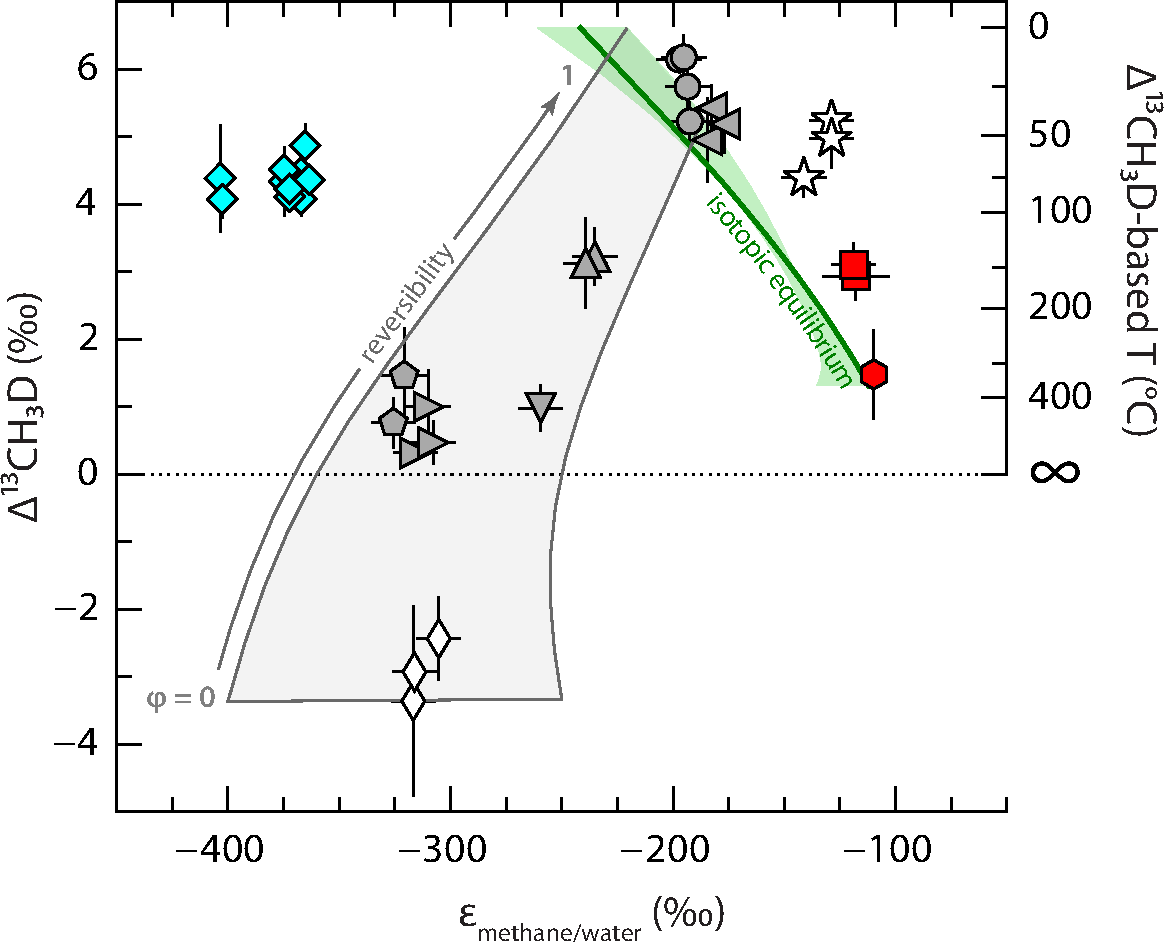
\includegraphics[width=0.5\linewidth]{figures/Fig2.2}
	\caption[Extent of clumped- and hydrogen-isotopic disequilibria in methane]{Extent of clumped- and hydrogen-isotopic disequilibria in methane. Symbols and vertical error bars are the same as those in \autoref{fig:2:1}.
	Horizontal error bars represent uncertainties on estimates of
	$\varepsilon$\textsubscript{methane/water}\footref{fn:2:epsilon} (\autoref{tab:2:S4}). The solid
	green curve represents isotopic equilibrium, with the
	$\varepsilon$\textsubscript{methane/water} calibration given by \textcite{Horibe+Craig_1995_GCA}. Green
	shading represents ranges of $\varepsilon$\textsubscript{methane/water} calibrations
	from published reports (\autoref{fig:2:S3}). Gray shading represents model
	predictions from this study for microbial methane formed between 0 and
	40~°C. Metabolic reversibility ($\varphi$) increases from bottom ($\varphi$ = 0,
	fully-kinetic) to top ($\varphi$ → 1, equilibrium) within this field
	(see \autoref{model-of-isotopologue-systematics-during-microbial-methanogenesis}).}
	\label{fig:2:2}
\end{SCfigure*}

\begin{SCfigure*}[][p]
	\centering
	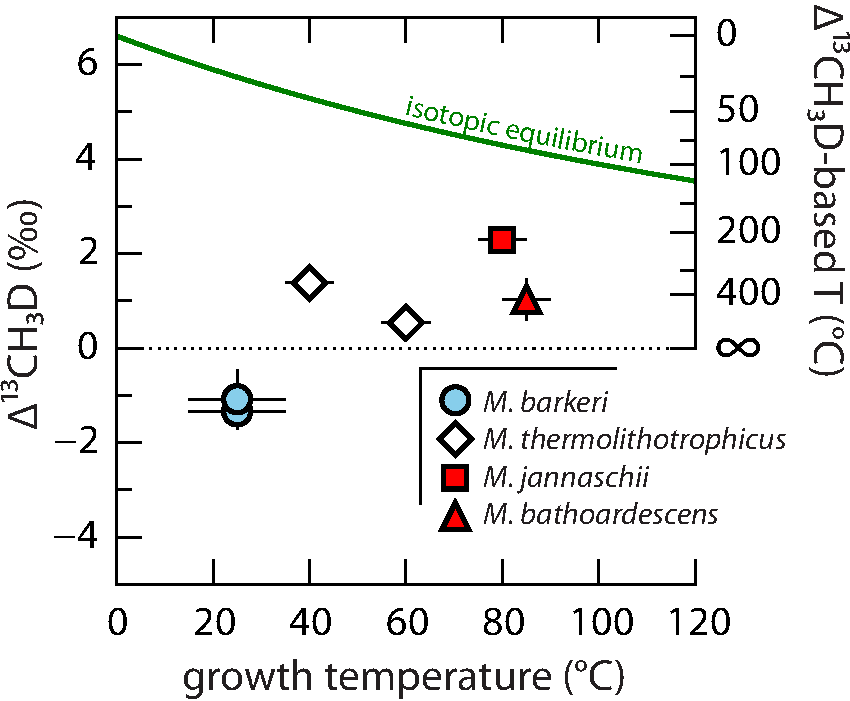
\includegraphics[width=0.37\linewidth]{figures/Fig2.3}
	\caption[Δ\textsuperscript{13}CH\textsubscript{3}D values of methane produced
	by hydrogenotrophic methanogens in batch cultures]{Δ\textsuperscript{13}CH\textsubscript{3}D values of me\-thane produced
		by hydro\-geno\-trophic methan\-ogens in batch cultures reflect kinetic
		effects. Data and error bars are from \autoref{tab:2:S2}. The green line
	represents clumped isotopologue equilibrium (i.e., samples for which
	Δ\textsuperscript{13}CH\textsubscript{3}D temperature is equal to growth
	temperature; \autoref{fig:2:S1}).}
	\label{fig:2:3}
\end{SCfigure*}
\begin{SCfigure*}[][p]
	\centering
	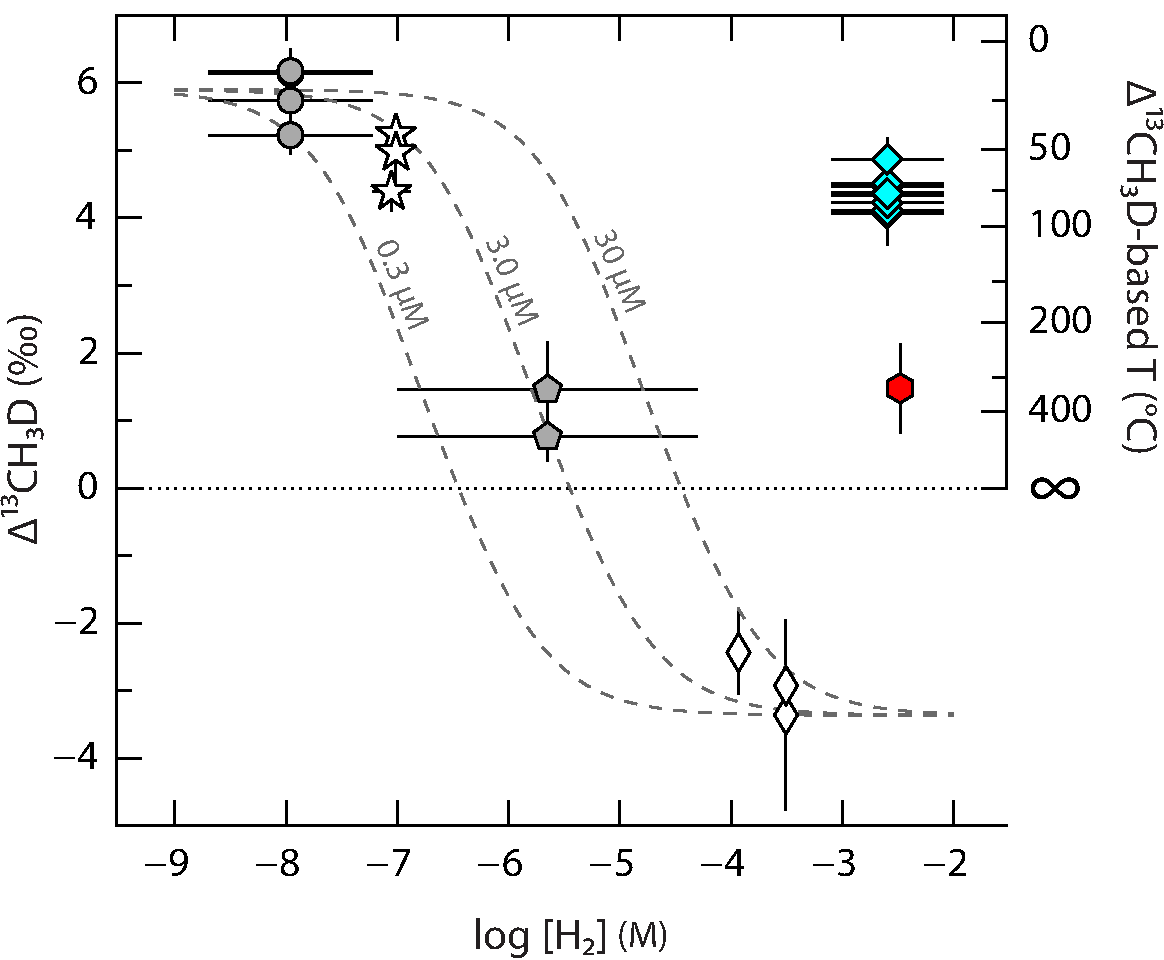
\includegraphics[width=0.5\linewidth]{figures/Fig2.4}
	\caption[Relationships between
	Δ\textsuperscript{13}CH\textsubscript{3}D and H\textsubscript{2}
	concentration for microbial methane]{Relationships between
		Δ\textsuperscript{13}CH\textsubscript{3}D and H\textsubscript{2}
		concentration for microbial methane. Symbols and vertical error bars
	are the same as in \autoref{fig:2:1}. The H\textsubscript{2} data are from \autoref{tab:2:S4}; when a range of {[}H\textsubscript{2}{]} values is given, points are
	plotted at the geometric mean of the maximum and minimum values. Dashed
	lines represent model predictions for microbial methane produced at 20~°C, calculated using \emph{K}\textsubscript{M}'s of 0.3, 3.0, and 30~µM
	H\textsubscript{2}. Data for samples of dominantly non-microbial methane
	from Guaymas Basin and Kidd Creek are plotted for comparison.}
	\label{fig:2:4}
\end{SCfigure*}


Despite the similarity in geologic setting, methane associated with
serpentinization at CROMO \parencite{Cardace++_2013_SD} revealed very different
Δ\textsuperscript{13}CH\textsubscript{3}D values that correspond to
low apparent temperatures (42--76~°C) and plot close to the equilibrium
line (\autoref{fig:2:2}). While the conventional δ\textsuperscript{13}C and δD
values of methane from CROMO are nearly identical to those of the Utica
Shale sample (\mrefs[B]{Fig.}{fig:2:1}), methane at CROMO carries much higher
Δ\textsuperscript{13}CH\textsubscript{3}D values (\mrefs[A]{Fig.}{fig:2:1}). The origin
of methane at the CROMO site remains unresolved \parencite{Cardace++_2013_SD}, but the
comparably high Δ\textsuperscript{13}CH\textsubscript{3}D values at
CROMO suggest that methane here could be sourced from a mixture of
thermogenic and microbial methane. Alternatively, lower
H\textsubscript{2} availability at CROMO compared to The Cedars (\autoref{tab:2:S4}), may support microbial methanogenesis under near-equilibrium
conditions (\autoref{fig:2:4}). Regardless, the different isotopologue signatures
in methane from CROMO vs.\ The Cedars demonstrate that distinct processes
contribute to methane formation in these two serpentinization systems.

Deep, ancient fracture fluids in the Kidd Creek mine in the Canadian
Shield \parencite{Holland++_2013_N} contain copious quantities of both dissolved methane
and hydrogen \parencite{SherwoodLollar++_2002_N}. The Kidd Creek methane occupies a distinct
region in the Δ\textsuperscript{13}CH\textsubscript{3}D vs.\ $\varepsilon$\textsubscript{methane/water} diagram (\autoref{fig:2:2}), due to strong D/H
disequilibria between methane and water \parencite{SherwoodLollar++_2008_GCA} and low
Δ\textsuperscript{13}CH\textsubscript{3}D temperature signals of 56--90~°C that are consistent with other temperature estimates for these
groundwaters \parencite{SherwoodLollar++_2008_GCA}. Although the specific mechanisms by which the
proposed abiotic hydrocarbons at Kidd Creek are generated remain under
investigation \parencite{SherwoodLollar++_2002_N,SherwoodLollar++_2014_N}, the distinct isotopologue signals
provide further support for the hypothesis that methane here is neither
microbial nor thermogenic.

Our results demonstrate that measurements of
\textsuperscript{13}CH\textsubscript{3}D provide information beyond the
simple formation temperature of methane. The combination of methane/water
D/H fractionation and
\textsuperscript{13}CH\textsubscript{3}D abundance enables the
differentiation of methane that has been formed at extremely low rates
in the subsurface \parencite{Pohlman++_2009_EPSL,Bates++_2011_CG,Holler++_2011_PNAS} from methane formed
in cattle and surface environments in which methanogenesis proceeds at
comparatively high rates \parencite{Johnson+Johnson_1995_JAnimalSci,Varadharajan+Hemond_2012_JGR}.
\blfootnote{\textsc{note added during thesis preparation}: I do not favor the use of the term \emph{formation temperature}. 
This term has a distinct and widely-accepted meaning in industries associated with subsurface resources (particularly within the disciplines
of formation evaluation, reservoir engineering, and petrophysics).  Practitioners of isotope geochemistry can better communicate by using 
less-ambiguous wording such as \emph{temperatures of methane generation} and \emph{clumped isotopologue temperatures}. 
The distinction between these two concepts is important because---as this thesis demonstrates---apparent temperatures 
derived from equilibria between methane isotopologues are often different from the temperatures at which methane 
was generated.  Methane may also be generated at one temperature, and later ``scrambled'' (its C--H bonds 
rearranged/equilibrated) at a different temperature; only the temperature of last equilibration would be 
recorded by Δ\textsuperscript{13}CH\textsubscript{3}D values.} 
 %This approach provides
%a new window for interrogating the biochemistry of methanogenesis in
%nature.

\clearpage



\section{Acknowledgments}\label{acknowledgments}
%\textbf{Acknowledgments.} 
%\addcontentsline{toc}{section}{Acknowledgments}
We thank J. Hayes, R. Summons, A. Whitehill, S. Zaarur, C. Ruppel, L.T.
Bryndzia, N. Blair, D. Vinson, K. Nealson, and M. Schrenk for
discussions; W. Olszewski, D. Nelson, G. Lacrampe-Couloume, and B.
Topçuoğlu for technical assistance; A. Whitehill, G. Luo, A. Apprill, K.
Twing, W. Brazelton, A. Wray, J. Oh, A. Rowe, G. Chadwick, and A. Rietze
for assistance in the field; R. Michener for the δD\textsubscript{water}
analyses; and R. Dias (USGS) for sharing the NGS samples. We thank R.
Raiche and D. McCrory, S. Moore (Homestake Mining Co.) and the staff of
the McLaughlin Natural Reserve, and Shell and other operators for access
to samples. Grants from the National Science Foundation (EAR-1250394 to
S.O. and EAR-1322805 to J.C.M.), N. Braunsdorf and D. Smit of Shell
PTI/EG (to S.O.), the Deep Carbon Observatory (to S.O., B.S.L., M.K.,
and K.-U.H.), the Natural Sciences and Engineering Research Council of
Canada (to B.S.L.), and the Gottfried Wilhelm Leibniz Program of the
Deutsche Forschungsgemeinschaft (HI 616-14-1 to K.-U.H. and M.K.)
supported this study. D.T.W. was supported by a National Defense Science
and Engineering Graduate Fellowship. D.S.G. was supported by the Neil
and Anna Rasmussen Foundation Fund, the Grayce B. Kerr Fellowship, and a
Shell-MITEI Graduate Fellowship. Any use of trade, firm, or product
names is for descriptive purposes only and does not imply endorsement by
the U.S. Government.

%\textbf{Author Contributions.} 
\section*{Author Contributions}
D.T.W. and S.O. developed the methods,
analyzed data, and performed modeling. D.T.W. and D.S.G. performed
isotopic analyses. D.S.G., L.C.S., J.F.H., M.K., K.-U.H., and S.O.
designed and/or conducted microbiological experiments. D.T.W., D.S.G.,
B.S.L., P.L.M., K.B.D., A.N.H., C.N.S., M.D.K., D.J.R., J.C.M., D.C.,
and S.O. designed and/or executed the field sampling campaigns. D.T.W.
and S.O. wrote the manuscript with input from all authors.
%



\begin{landscape}	
	\begin{ThreePartTable}		
		\begin{TableNotes}
			\item Abbreviations: NCM, Northern Cascadia Margin; PRB, Powder River Basin;
			Swamp Y, Atlantic White Cedar Swamp; UML, Upper Mystic Lake; LML, Lower
			Mystic Lake; NAB, Northern Appalachian Basin; CROMO, Coast Range
			Ophiolite Microbial Observatory.
			
			\item * Purified sample was measured twice. The uncertainties reported for
			these samples are 95\% confidence intervals calculated from the data for
			each measurement (with $\sigma$ taken as the larger of 1\emph{s} or 0.3‰, which
			is typical analytical reproducibility) assuming the measurements follow
			a normal distribution.
			
			\item † Sample was subsampled, purified and analyzed twice (3 weeks apart) as
			described in the \autoref{field-site-descriptions-and-sampling-methods}. The uncertainties reported for this
			sample are 2~s.e.m. (standard error of the mean) of the replicate
			measurements (\emph{n} = 2).
			
			\item ‡ Sample was subsampled, purified and analyzed three times over a period
			of \textgreater{}3 months. The uncertainties reported for this sample
			are 2 s.e.m. of the replicate measurements (\emph{n} = 3).
		\end{TableNotes}
	
		\setlength{\tabcolsep}{10pt}
		\small
		\begin{longtable}[]{ll r@{\hspace{0.2em}}l r@{\hspace{0.2em}}l r@{\hspace{0.2em}}l r@{\hspace{0.2em}}l}
			
			\caption[Results of isotopic measurements of natural samples of
			methane]{Results of isotopic measurements of natural samples of
				methane. Uncertainties reported are 95\% confidence intervals over all
				measurement cycles for a single analysis. Values for
				δ\textsuperscript{13}C, δD, and
				Δ\textsuperscript{13}CH\textsubscript{3}D are reported relative to PDB,
				SMOW, and the stochastic distribution, respectively. Samples for which
				Δ\textsuperscript{13}CH\textsubscript{3}D is $\leq$ 0‰ have no corresponding
				thermodynamically-allowed apparent equilibrium temperature (\textit{T}\textsubscript{13D}), and are
				noted as anti-clumped (a.c.).}\label{tab:2:S1}\\	% this \\ is very important !!
			\toprule
			Sample Set & Sample Name & \multicolumn{2}{c}{δ\textsuperscript{13}C (‰)} & \multicolumn{2}{c}{δD (‰)} &
			\multicolumn{2}{c}{Δ\textsuperscript{13}CH\textsubscript{3}D (‰)} & \multicolumn{2}{c}{\textit{T}\textsubscript{13D}
			(°C)}\tabularnewline
			\midrule
			\endfirsthead
			
			\caption[]{Results of isotopic measurements of natural samples of
				methane (\textit{continued}).}\\
			\toprule
			Sample Set & Sample Name & \multicolumn{2}{c}{δ\textsuperscript{13}C (‰)} & \multicolumn{2}{c}{δD (‰)} &
			\multicolumn{2}{c}{Δ\textsuperscript{13}CH\textsubscript{3}D (‰)} & \multicolumn{2}{c}{\textit{T}\textsubscript{13D}
				(°C)}\tabularnewline
			\midrule
			\endhead
			
			\midrule
			\multicolumn{10}{r}{\textit{Continued on next page}}
			\endfoot
			
%			\multicolumn{10}{l}{\small Abbreviations: NCM, Northern Cascadia Margin; PRB, Powder River Basin;
%				Swamp Y, Atlantic White Cedar Swamp; UML, Upper Mystic Lake; LML, Lower
%				Mystic Lake; NAB, Northern Appalachian Basin; CROMO, Coast Range
%				Ophiolite Microbial Observatory.}
%			\multicolumn{10}{l}{
%				* Purified sample was measured twice. The uncertainties reported for
%				these samples are 95\% confidence intervals calculated from the data for
%				each measurement (with $\sigma$ taken as the larger of 1\emph{s} or 0.3‰, which
%				is typical analytical reproducibility) assuming the measurements follow
%				a normal distribution.\\				
%				† Sample was subsampled, purified and analyzed twice (3 weeks apart) as
%				described in the \emph{SI Text}. The uncertainties reported for this
%				sample are 2 s.e.m. (standard error of the mean) of the replicate
%				measurements (\emph{n} = 2).\\				
%				‡ Sample was subsampled, purified and analyzed three times over a period
%				of \textgreater{}3 months. The uncertainties reported for this sample
%				are 2 s.e.m. of the replicate measurements (\emph{n} = 3).
%		}
			\insertTableNotes\\
			\endlastfoot
			
			\tabularnewline
			Bovine Rumen & Sally-1* & \textbf{$-$52.81} & ± 0.04 & \textbf{$-$342.56}
			& ± 0.04 & \textbf{1.46} & ± 0.71 & \textbf{330} & +190/$-$101
			\tabularnewline
			& Sally-2-5* & \textbf{$-$54.15} & ± 0.07 & \textbf{$-$347.25} & ± 0.07
			& \textbf{0.76} & ± 0.49 & \textbf{515} & +309/$-$144 \tabularnewline
			
			\tabularnewline
			NCM & 311-1325B-19X-4 (145-146) / Void, SB & \textbf{$-$68.50} & ± 0.10
			& \textbf{$-$189.48} & ± 0.10 & \textbf{5.74} & ± 0.49 & \textbf{25} &
			+16/$-$15 \tabularnewline
			& 311-1325C-6X-4 (17-18) / Void, SB & \textbf{$-$67.63} & ± 0.07 &
			\textbf{$-$188.40} & ± 0.07 & \textbf{5.22} & ± 0.29 & \textbf{42} &
			+11/$-$10 \tabularnewline
			& 311-1328E-2X-CC (0-10) / Hyd, SB & \textbf{$-$63.14} & ± 0.04 &
			\textbf{$-$193.26} & ± 0.04 & \textbf{6.14} & ± 0.21 & \textbf{13} &
			+6/$-$6 \tabularnewline
			& 311-1328E-2X-CC (0-10) / Hyd, Vac & \textbf{$-$61.63} & ± 0.08 &
			\textbf{$-$191.14} & ± 0.08 & \textbf{6.17} & ± 0.34 & \textbf{12} &
			+10/$-$9 \tabularnewline
			
			\tabularnewline
			PRB & DR\_15W-17-08-41 & \textbf{$-$59.74} & ± 0.08 & \textbf{$-$292.75} &
			± 0.12 & \textbf{5.42} & ± 0.34 & \textbf{35} & +12/$-$11
			\tabularnewline
			& DR\_3CA34 & \textbf{$-$62.03} & ± 0.10 & \textbf{$-$290.80} & ± 0.10 &
			\textbf{4.95} & ± 0.63 & \textbf{52} & +26/$-$22 \tabularnewline
			& DR\_Visborg\_13W-17-08-41 & \textbf{$-$58.58} & ± 0.10 &
			\textbf{$-$293.89} & ± 0.10 & \textbf{5.19} & ± 0.43 & \textbf{44} &
			+16/$-$15 \tabularnewline
			
			\tabularnewline
			Swamp Y & SwampY-1 & \textbf{$-$59.72} & ± 0.06 & \textbf{$-$322.17} & ±
			0.06 & \textbf{0.47} & ± 0.33 & \textbf{660} & +318/$-$159
			\tabularnewline
			& SwampY-2 & \textbf{$-$59.25} & ± 0.06 & \textbf{$-$324.27} & ± 0.06 &
			\textbf{1.00} & ± 0.55 & \textbf{435} & +238/$-$121 \tabularnewline
			& SwampY-5\textsuperscript{†} & \textbf{$-$59.70} & ± 0.32 &
			\textbf{$-$330.14} & ± 0.21 & \textbf{0.32} & ± 0.10 & \textbf{775} &
			+100/$-$78 \tabularnewline
			
			\tabularnewline
			UML & UML 06/19/2014 & \textbf{$-$70.96} & ± 0.10 & \textbf{$-$264.97} & ±
			0.10 & \textbf{3.22} & ± 0.43 & \textbf{139} & +32/$-$26
			\tabularnewline
			& UML 07/29/2014 & \textbf{$-$70.99} & ± 0.16 & \textbf{$-$268.93} & ±
			0.16 & \textbf{3.13} & ± 0.67 & \textbf{145} & +54/$-$41
			\tabularnewline
			
			\tabularnewline
			LML & LML-20m & \textbf{$-$65.47} & ± 0.07 & \textbf{$-$289.81} & ± 0.07
			& \textbf{0.98} & ± 0.35 & \textbf{440} & +133/$-$87 \tabularnewline
			
			\tabularnewline
			The Cedars & The Cedars NS, 2013 June & \textbf{$-$67.97} & ± 0.12 &
			\textbf{$-$333.06} & ± 0.07 & \textbf{$-$2.43} & ± 0.62 & \textbf{a.c.}
			&\tabularnewline
			& The Cedars BSC, 2013 June & \textbf{$-$63.81} & ± 0.21 &
			\textbf{$-$341.98} & ± 0.16 & \textbf{$-$3.36} & ± 1.42 & \textbf{a.c.}
			&\tabularnewline
			& The Cedars BSC, 2014 July & \textbf{$-$64.39} & ± 0.05 &
			\textbf{$-$341.48} & ± 0.05 & \textbf{$-$2.93} & ± 0.24 & \textbf{a.c.}
			&\tabularnewline
			
			\tabularnewline
			NAB & Marcellus Fm. & \textbf{$-$36.18} & ± 0.09 & \textbf{$-$157.60} & ±
			0.07 & \textbf{3.10} & ± 0.33 & \textbf{147} & +25/$-$22
			\tabularnewline
			& Utica Fm. & \textbf{$-$25.70} & ± 0.08 & \textbf{$-$153.10} & ± 0.08 &
			\textbf{2.93} & ± 0.36 & \textbf{160} & +29/$-$25 \tabularnewline
			
			\tabularnewline
			Guaymas & Rebecca's Roost 4462-IGT4, VT1 & \textbf{$-$43.96} & ± 0.18 &
			\textbf{$-$106.24} & ± 0.16 & \textbf{1.48} & ± 0.67 & \textbf{326} &
			+170/$-$95 \tabularnewline
			
			\tabularnewline
			\tabularnewline
			CROMO & CROMO-CSWold & \textbf{$-$26.98} & ± 0.07 & \textbf{$-$169.56} & ±
			0.07 & \textbf{4.39} & ± 0.29 & \textbf{76} & +14/$-$12
			\tabularnewline
			& CROMO-N08-A.1 & \textbf{$-$26.39} & ± 0.07 & \textbf{$-$157.53} & ± 0.06
			 & \textbf{5.24} & ± 0.31 & \textbf{42} & +11/$-$10 \tabularnewline
			& CROMO-N08-A.2 & \textbf{$-$26.55} & ± 0.12 & \textbf{$-$157.50} & ± 0.13
			 & \textbf{4.97} & ± 0.44 & \textbf{52} & +18/$-$16 \tabularnewline
			 
			\tabularnewline
			Kidd Creek & 14.06.2012.KC.L9500\_BHY13762\_Gas D & \textbf{$-$32.66} & ±
			0.07 & \textbf{$-$420.74} & ± 0.07 & \textbf{4.38} & ± 0.80 &
			\textbf{76} & +41/$-$32 \tabularnewline
			& 29.11.2012.KC.L9500\_BH2\_Gas C & \textbf{$-$32.28} & ± 0.07 &
			\textbf{$-$419.74} & ± 0.06 & \textbf{4.07} & ± 0.29 & \textbf{90} &
			+15/$-$14 \tabularnewline
			& KC\_12.02.2008\_7850L\_BH12299(E) & \textbf{$-$39.11} & ± 0.11 &
			\textbf{$-$397.33} & ± 0.05 & \textbf{4.51} & ± 0.25 & \textbf{70} &
			+11/$-$10 \tabularnewline
			& KC\_12.01.2010\_7850L\_BH12299(F) & \textbf{$-$39.73} & ± 0.06 &
			\textbf{$-$397.39} & ± 0.06 & \textbf{4.34} & ± 0.52 & \textbf{78} &
			+26/$-$22 \tabularnewline
			& KC\_01.03.2012\_7850L\_BH12299(F)\textsuperscript{‡} & \textbf{$-$40.19}
			& ± 0.05 & \textbf{$-$394.98} & ± 0.03 & \textbf{4.11} & ± 0.37 &
			\textbf{89} & +19/$-$17 \tabularnewline
			& 02.04.2014\_KC\_7850L\_BH12299(C) & \textbf{$-$39.72} & ± 0.04 &
			\textbf{$-$390.12} & ± 0.03 & \textbf{4.47} & ± 0.22 & \textbf{72} &
			+10/$-$9 \tabularnewline
			& 02.04.2014\_KC\_7850L\_BH12299(D) & \textbf{$-$39.72} & ± 0.06 &
			\textbf{$-$390.12} & ± 0.06 & \textbf{4.07} & ± 0.26 & \textbf{90} &
			+13/$-$12 \tabularnewline
			& KC\_27.08.2007\_7850L\_BH12287A(C) & \textbf{$-$40.64} & ± 0.04 &
			\textbf{$-$386.48} & ± 0.05 & \textbf{4.36} & ± 0.22 & \textbf{77} &
			+10/$-$10 \tabularnewline
			& KC\_20.06.2008\_7850L\_BH12287A(D) & \textbf{$-$40.25} & ± 0.08 &
			\textbf{$-$395.07} & ± 0.05 & \textbf{4.23} & ± 0.30 & \textbf{83} &
			+15/$-$13 \tabularnewline
			& KC\_20.09.2013\_7850L\_BH12287A(B) & \textbf{$-$41.44} & ± 0.06 &
			\textbf{$-$388.32} & ± 0.06 & \textbf{4.87} & ± 0.32 & \textbf{56} &
			+13/$-$12 \tabularnewline
			
			\tabularnewline
			\bottomrule
		\end{longtable}
%		\noindent \small Abbreviations: NCM, Northern Cascadia Margin; PRB, Powder River Basin;
%		Swamp Y, Atlantic White Cedar Swamp; UML, Upper Mystic Lake; LML, Lower
%		Mystic Lake; NAB, Northern Appalachian Basin; CROMO, Coast Range
%		Ophiolite Microbial Observatory.
%	
%		\noindent * Purified sample was measured twice. The uncertainties reported for
%		these samples are 95\% confidence intervals calculated from the data for
%		each measurement (with $\sigma$ taken as the larger of 1\emph{s} or 0.3‰, which
%		is typical analytical reproducibility) assuming the measurements follow
%		a normal distribution.
%		
%		\noindent † Sample was subsampled, purified and analyzed twice (3 weeks apart) as
%		described in the \emph{SI Text}. The uncertainties reported for this
%		sample are 2 s.e.m. (standard error of the mean) of the replicate
%		measurements (\emph{n} = 2).
%		
%		\noindent ‡ Sample was subsampled, purified and analyzed three times over a period
%		of \textgreater{}3 months. The uncertainties reported for this sample
%		are 2 s.e.m. of the replicate measurements (\emph{n} = 3).
				
	\end{ThreePartTable}
\end{landscape}




\section{Materials and Methods}\label{materials-and-methods}

\subsection{Animal care }\label{animal-care}

Sampling of methane from bovine subjects was conducted according to
guidelines established by the Institutional Animal Care and Use
Committee at the Pennsylvania State University.

\subsection{Cultivation of methanogens
}\label{cultivation-of-methanogens}

We established batch culture incubations of \emph{Methanocaldococcus
bathoardescens}, \emph{Methanocaldococcus jannaschii}, \emph{Methanothermococcus
thermolithotrophicus}, and \emph{Methanosarcina barkeri} under atmospheres
containing 80\% H\textsubscript{2} and 20\% CO\textsubscript{2}.
Cultures of \emph{M. jannaschii} \parencite{Jones++_1983_AoM} and \emph{M. barkeri} (strain DSM-800) \parencite{Balch++_1979_MR} were
purchased from the German Collection of Microorganisms and Cell Cultures
(DSMZ, Braunschweig, Germany). \emph{Methanocaldococcus bathoardescens}
(formerly known as strain JH146) is a recently-isolated
hyperthermophilic, obligate hydrogenotrophic methanogen exhibiting
optimum growth at 82~°C \parencite{Stewart++_2015_IJSEM,VerEecke++_2013_EMR}. The growth medium for \emph{M. jannaschii}, \emph{M.
thermolithotrophicus}, and \emph{M. bathoardescens} was prepared according to
the recipe for DSMZ medium 282, amended with 1~g/L
NaS\textsubscript{2}O\textsubscript{3}. Aliquots of the medium (50 ml)
were transferred into 160 ml glass serum vials stoppered with blue butyl
rubber septa, and the headspace was filled with 2 atm
H\textsubscript{2}:CO\textsubscript{2} (80:20). The growth medium for \emph{M.
barkeri} was prepared according to the recipe for DSMZ medium 120, and
the headspace was filled with 1.5 atm
H\textsubscript{2}:CO\textsubscript{2} (80:20). Cultures were incubated
at ambient temperature (\emph{M. barkeri}, in duplicate), at 40 and 60~°C (\emph{M.
thermolithotrophicus}), at 80~°C (\emph{M. jannaschii}), or at 85~°C (\emph{M.
bathoardescens}).


\begin{sidewaystable}\centering
	\begin{threeparttable}
		\caption[Results of isotopic measurements of methane produced
		in batch cultures of methanogens]{Results of isotopic measurements of methane produced
			experimentally by cultures of methanogens. Each line represents a
		separate bottle incubation of an axenic strain of methanogens.
		Uncertainties reported are 95\% confidence intervals over all
		measurement cycles for a single analysis. Values for
		δ\textsuperscript{13}C, δD, and
		Δ\textsuperscript{13}CH\textsubscript{3}D are reported relative to PDB,
		SMOW, and the stochastic distribution, respectively. Samples for which
		Δ\textsuperscript{13}CH\textsubscript{3}D $\leq$ 0‰ have no corresponding
		thermodynamically-allowed apparent equilibrium temperature, and are
		noted as anti-clumped (a.c.).}
		\label{tab:2:S2}
		
		\small
		\begin{tabular}{ll r@{\hspace{0.2em}}l r@{\hspace{0.2em}}l r@{\hspace{0.2em}}l r@{\hspace{0.2em}}l}
			\toprule
			Culture & growth T* & \multicolumn{2}{c}{δ\textsuperscript{13}C (‰)} & \multicolumn{2}{c}{δD (‰)} &
			\multicolumn{2}{c}{Δ\textsuperscript{13}CH\textsubscript{3}D (‰)} & \multicolumn{2}{c}{\textit{T}\textsubscript{13D}
				(°C)}\tabularnewline
			\midrule
			\emph{Methanocaldococcus bathoardescens} & 85~°C & \textbf{$-$12.58} & ±
			0.07  & \textbf{$-$419.23} & ± 0.07  & \textbf{1.03} & ± 0.45  &
			\textbf{426} & +170/$-$100 \tabularnewline
			\emph{Methanocaldococcus jannaschii} & 80~°C & \textbf{$-$18.79} & ± 0.03
			 & \textbf{$-$416.90} & ± 0.05  & \textbf{2.29} & ± 0.23  &
			\textbf{216} & +25/$-$22 \tabularnewline
			\emph{Methanothermococcus thermolithotrophicus} & 60~°C &
			\textbf{$-$17.05} & ± 0.05  & \textbf{$-$409.84} & ± 0.05  & \textbf{0.54}
			& ± 0.28  & \textbf{620} & +214/$-$126 \tabularnewline
			\emph{Methanothermococcus thermolithotrophicus} & 40~°C &
			\textbf{$-$16.47} & ± 0.04  & \textbf{$-$427.76} & ± 0.04  & \textbf{1.38}
			& ± 0.34  & \textbf{345} & +79/$-$58 \tabularnewline
			\emph{Methanosarcina barkeri} & ambient & \textbf{$-$59.90} & ± 0.05  &
			\textbf{$-$418.40} & ± 0.05  & \textbf{$-$1.34} & ± 0.22  & \textbf{a.c.}
			&\tabularnewline
			\emph{Methanosarcina barkeri } & ambient & \textbf{$-$50.30} & ± 0.07  &
			\textbf{$-$422.67} & ± 0.07  & \textbf{$-$1.08} & ± 0.63  & \textbf{a.c.}
			&\tabularnewline
			\bottomrule
		\end{tabular}
		{\small * Uncertainty on measured growth temperatures is estimated at ±5~°C.
			Temperatures were not monitored throughout the \emph{M. barkeri}
			incubations but are estimated at 25 ± 10~°C.}

	\end{threeparttable}
\end{sidewaystable}



\subsection{Sample purification procedures
}\label{sample-purification-procedures}


\begin{figure*}
	\centering
	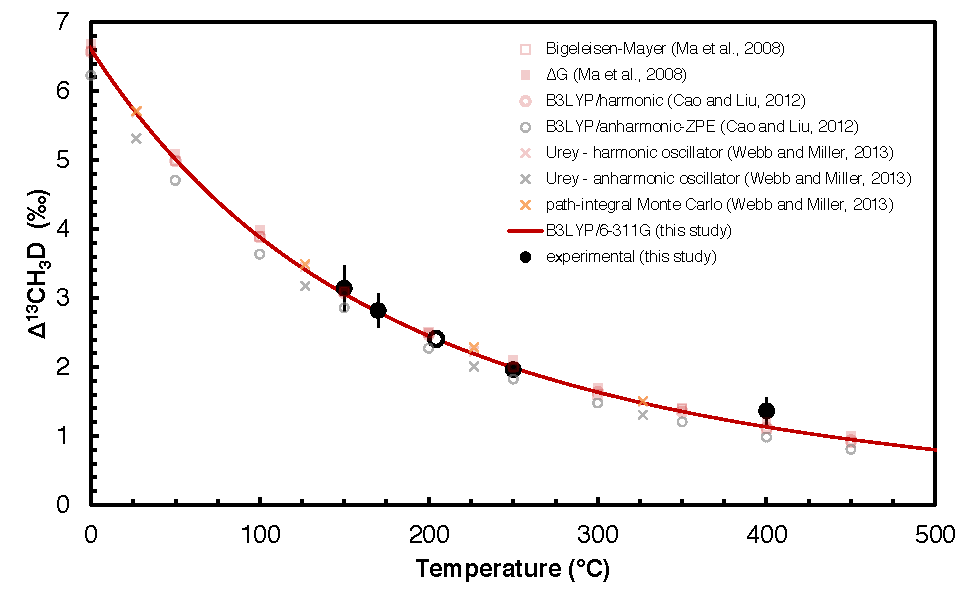
\includegraphics[width=0.8\linewidth]{figures/Fig2.S1}
	\caption[Experimental calibration of the
	Δ\textsuperscript{13}CH\textsubscript{3}D thermometer]{Experimental calibration of the
		Δ\textsuperscript{13}CH\textsubscript{3}D thermometer. Filled circles
	represent the mean Δ\textsuperscript{13}CH\textsubscript{3}D of gases
	heated at that temperature, and error bars represent 95\% confidence
	intervals calculated from a normal distribution (for the 150~°C sample,
	error bars represent the 95\% confidence interval on the measurement
	cycles in a single analysis, calculated from a \emph{t}-distribution).
	For the 250~°C point, the error bars are smaller than the symbol. The
	open circle represents our reference gas, AL1. The equilibrium curve
	(red line) was calculated following conventional equilibrium isotope
	fractionation theory under the harmonic oscillator assumption
	\parencite{Bigeleisen+Mayer_1947_JCP}; frequencies were calculated at the B3LYP level of theory
	using the 6-311G basis set as implemented in Gaussian 03 (\citeauthor{g03}).
	For comparison, results from published computational studies
	\parencite{Webb+Miller_2013_JPCA,Cao+Liu_2012_GCA,Ma++_2008_GCA} are also plotted.}
	\label{fig:2:S1}
\end{figure*}

\begin{figure*}
	\centering
	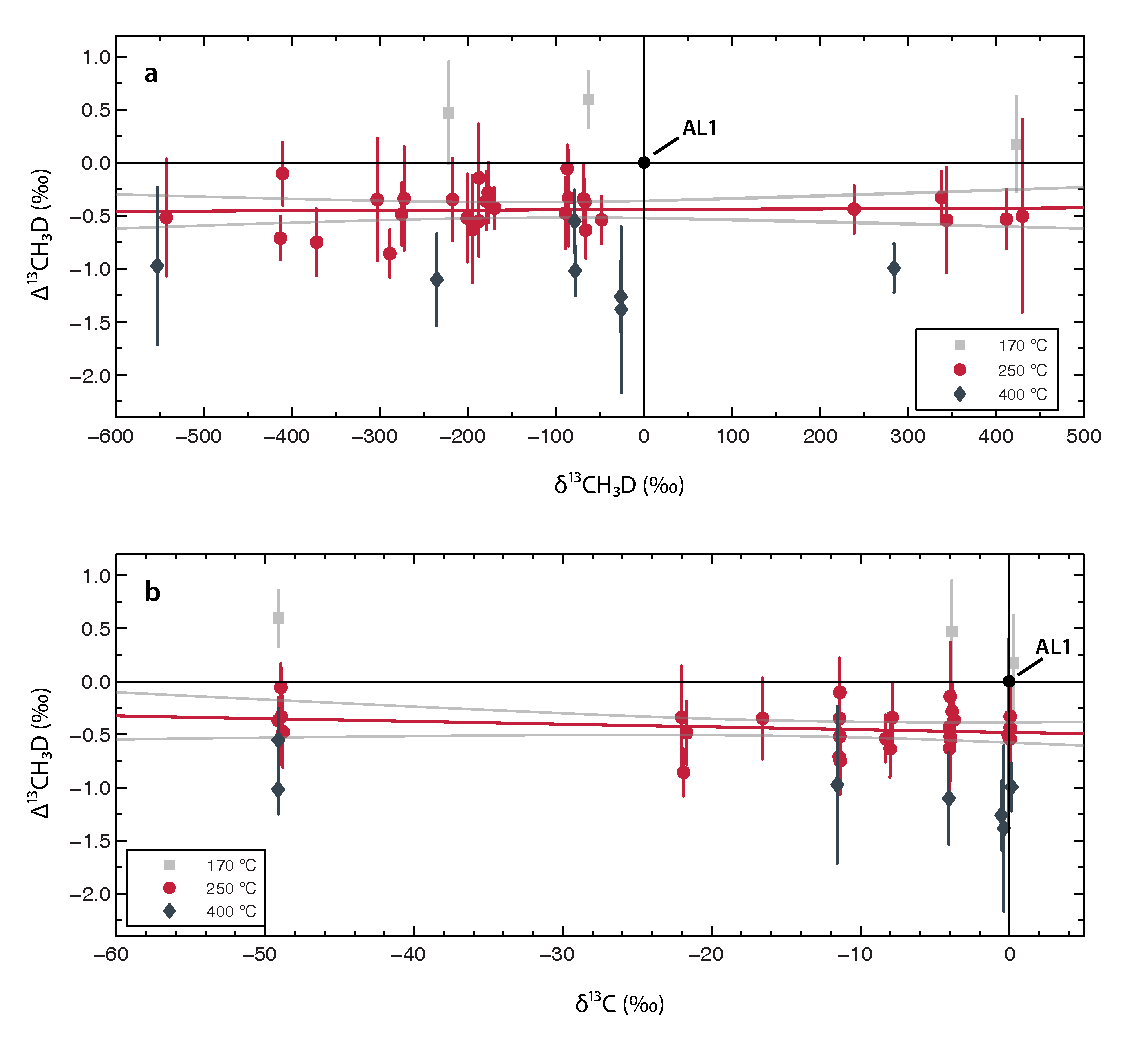
\includegraphics[width=0.85\linewidth]{figures/Fig2.S2}
	\caption[Demonstration of linearity in Δ\textsuperscript{13}CH\textsubscript{3}D over a range of bulk isotope ratios]{Demonstration of linearity in Δ\textsuperscript{13}CH\textsubscript{3}D over a range of bulk isotope ratios.  Shown are measurements of methane heated over catalyst at three
		temperatures (170, 250, 400~°C).  Solid red lines represent unweighted linear least squares
	regressions through gases equilibrated at 250~°C, and gray lines denote
	the 95\% confidence band. Error bars represent 95\% confidence intervals
	on multiple measurement cycles of a single analysis. Isotopic ratios are
	shown relative to our reference gas, AL1. Results indicate no
	significant correlation between
	Δ\textsuperscript{13}CH\textsubscript{3}D and (\textbf{A})
	δ\textsuperscript{13}CH\textsubscript{3}D over an 800‰ range (the
	variation in δ\textsuperscript{13}CH\textsubscript{3}D is driven mainly
	by differences in δD); and (\textbf{B}) δ\textsuperscript{13}C over a
	48‰ range.}
	\label{fig:2:S2}
\end{figure*}


To extract methane quantitatively from gas samples, we applied a
preparative-gas chromatography technique modified from \textcite{Alei++_1987_AtmE}. In brief, a sample is introduced into a stream of helium.
Water is removed by passing the sample through a U-trap cooled to $-$80~°C, and then CH\textsubscript{4}, air (N\textsubscript{2},
O\textsubscript{2}, Ar), CO, CO\textsubscript{2}, and
C\textsubscript{2+} are cryofocused onto a U-trap packed with activated
charcoal and held at $-$196~°C. The condensed gases are then released by
rapid heating to 120~°C, passed through a packed column (Carboxen-1000,
5$'$ × 1/8$''$, Supelco) held at 30~°C under helium flow (\textasciitilde{}25
ml/min), and monitored using thermal conductivity detection. The methane
peak is trapped on a U-trap packed with silica gel and held at $-$196~°C;
this is analogous to a ``heart-cut'' technique used previously for
preparative separation of SF\textsubscript{6} for isotopic analysis
\parencite{Ono++_2006_CG}. After elution of methane, the column is baked at 180~°C
under a reversed (backflushed) flow of helium to remove
CO\textsubscript{2} and C\textsubscript{2+}.

This sample preparation procedure induces small fractionations in
δ\textsuperscript{13}C and δD of methane of 0.09 ± 0.06‰ and 0.20 ±
0.02‰, respectively (1\emph{s}, \emph{n} = 4); these effects are minor
compared to the magnitude of δ\textsuperscript{13}C and δD variations in
nature. Critically, our procedure does not discernibly alter the
Δ\textsuperscript{13}CH\textsubscript{3}D value; the average difference
between samples treated vs.\ not treated with this procedure was $-$0.09 ±
0.16‰ (1\emph{s}, \emph{n} = 4), which is not significantly different
from zero.

\subsection{\texorpdfstring{Reporting of δ\textsuperscript{13}C and δD
		values}{Reporting of δ13C and δD
		values}}\label{reporting-of-ux3b413c-and-ux3b4d-values}

The δ\textsuperscript{13}C and δD values we report have been calibrated
relative to PDB and SMOW, respectively, by measuring samples of NGS-1
and NGS-3. These reference values for δ\textsuperscript{13}C and δD are,
respectively, $-$29.0‰ and $-$138‰ for NGS-1, and $-$72.8‰ and $-$176‰ for
NGS-3, as determined by several labs in the 1980s \parencite{Hut_1987}. Results for the calibration
samples are shown in \autoref{tab:2:S5}.

\subsection{Heated gas calibrations}\label{heated-gas-calibrations}

To confirm and extend a previously-published temperature calibration
\parencite{Ono++_2014_AC}, Pyrex tubes containing samples of methane with a range of
δ\textsuperscript{13}C ($-$82 to $-$34‰ vs.\ PDB) and δD ($-$615 to +220‰ vs.\ SMOW) were prepared. These samples were heated over Pt catalyst at
temperatures of 150, 170, 250, and 400~°C (\emph{n} = 1, 3, 28, and 7,
respectively). Gases were heated for 110 d, 73--76 d, 2--24 d, and
16--60 h, respectively, following a procedure described in 
\textcite{Ono++_2014_AC}.

When the theoretical methane equilibrium line is aligned to samples
heated at 150, 170, and 250~°C, measurements of the samples heated at
400~°C yielded slightly lower Δ\textsuperscript{13}CH\textsubscript{3}D
temperatures
($347^{+42}_{-36}$\,°C),
perhaps because quenching the reaction may take longer than the time for
exchange over catalyst at \textasciitilde{}400~°C. As a result, the data
from the 400~°C heated gases were not used in aligning the calibration
in \autoref{fig:2:S1}.

The theoretical equilibrium line we calculated agrees well with
published results from both path-integral Monte Carlo simulations
\parencite{Webb+Miller_2013_JPCA} and harmonic oscillator assumption-based approaches
\parencite{Webb+Miller_2013_JPCA,Cao+Liu_2012_GCA,Ma++_2008_GCA}. The results of results of calculations employing
an anharmonic correction, however, differ slightly from results of
models assuming harmonic-oscillator behavior \parencite[by \textasciitilde{}0.3‰
near room temperature;][]{Webb+Miller_2013_JPCA,Cao+Liu_2012_GCA}. \mrefs[]{Figure}{fig:2:S1} shows results
from recent studies comparing multiple
computational approaches for estimating the temperature-dependence of
the equilibrium Δ\textsuperscript{13}CH\textsubscript{3}D value. We note
that while the uncertainty in the theoretical curve is similar in
magnitude to our analytical uncertainty, particularly at temperatures
\textless{}100~°C, these calibration uncertainties do not affect the
conclusions drawn in this study.

\subsection{Spectroscopic procedures
}\label{spectroscopic-procedures}

Samples of purified methane were analyzed using a tunable-infrared laser
direct absorption spectrometer (Aerodyne Research, Billerica,
Massachusetts) housed at MIT as described in \textcite{Ono++_2014_AC},
with improvements described here. All measurements reported in this
paper were obtained at a nominal cell pressure of ca.\ 1.0~Torr, instead
of the 0.8~Torr used in \textcite{Ono++_2014_AC}. We have found that this
higher cell pressure gave improved measurement stability. As suggested
previously \parencite{Ono++_2014_AC}, there is a small offset in the baseline
underneath the \textsuperscript{13}CH\textsubscript{3}D absorption line,
likely due to the insufficient accuracy of the Voigt profile for
describing the contribution from tailing of adjacent
\textsuperscript{12}CH\textsubscript{4} peak. We have used all 250~°C
experiments shown in \autoref{fig:2:S2} to generate a single set of correction
factors, which show no observable drift during the time period all
measurements were made.

Long-term internal reproducibility was evaluated by repeated analysis of
methane from a commercially-sourced gas cylinder over a period of
\textgreater{}4 months, yielding precisions for δ\textsuperscript{13}C
of ±0.02‰, δD of ±0.02‰, and Δ\textsuperscript{13}CH\textsubscript{3}D
of ±0.08‰ (1\emph{s}, \emph{n} = 13). As described in \textcite{Ono++_2014_AC}, each measurement run consists of multiple acquisition
cycles (a cycle is defined as one comparison of a sample/standard pair).
The number of cycles (\emph{N}\textsubscript{cycles}) depends on sample
size, but is typically greater than 5. In this paper,
Δ\textsuperscript{13}CH\textsubscript{3}D measurements are reported as
mean ± 95\% confidence intervals (CI) on the average of all isotope
ratios obtained for each acquisition cycle over a measurement run,
calculated as: 
$ \text{95\% CI} = \mathit{tinv}\left( \alpha,\mathit{df}\right) \cdot {s\,/\sqrt{\smash[b]{N_\text{cycles}}}} $, where $ \mathit{tinv} $ is the two-tailed inverse of the Student’s \textit{t}-distribution for $ \alpha = 0.05 $ with $ N_\text{cycles} - 1 $ degrees of freedom ($ \mathit{df} $), and $ s \geq 0.27\permille$
{[}this value is the
standard deviation on measurements for which 24 or more cycles were
taken (0.27 ± 0.08‰, 1\emph{s} on 1\emph{s}, \emph{n} = 7), and thus
estimates the internal precision of the instrument{]}. The uncertainties
on Δ\textsuperscript{13}CH\textsubscript{3}D values reported for samples
in \mrefs[]{Tables}{tab:2:S1}, \ref{tab:2:S2}, and \ref{tab:2:S5} also contain the propagated uncertainty in the
Δ\textsuperscript{13}CH\textsubscript{3}D value of our methane reference
gas (AL1). Based on the calibration shown in \autoref{fig:2:S1}, we determined that
AL1 carries a Δ\textsuperscript{13}CH\textsubscript{3}D value of +2.41 ±
0.08‰ (95\% CI).



\begin{figure*}
	\centering
	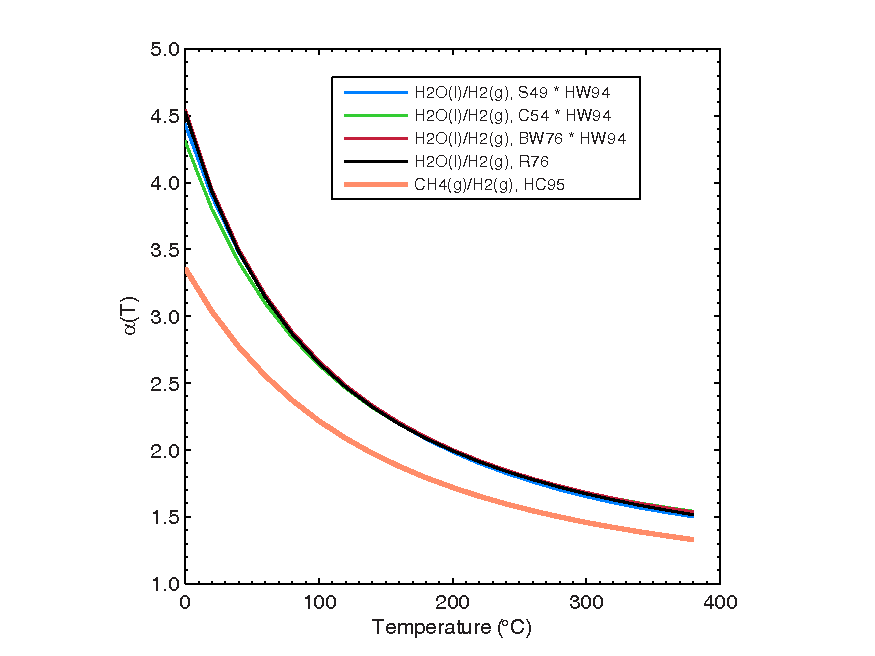
\includegraphics[width=0.8\linewidth]{figures/Fig2.S3}
	\caption[Equilibrium hydrogen isotopic fractionation factors
	for the system H\textsubscript{2}--H\textsubscript{2}O--CH\textsubscript{4}]{Equilibrium hydrogen isotopic fractionation factors
		compiled from experimental and theoretical calibrations. When
	appropriate, calibrations for
	H\textsubscript{2}O(g)/H\textsubscript{2}(g) have been converted using
	the H\textsubscript{2}O(l)/H\textsubscript{2}O(g) calibration from
	\textcite{Horita+Wesolowski_1994_GCA} to derive
	H\textsubscript{2}O(l)/H\textsubscript{2}(g) calibrations. 
	HW94, \textcite{Horita+Wesolowski_1994_GCA}; 
	S49, \textcite{Suess_1949}; 
	C54, \textcite{Cerrai++_1954}; 
	BW76, \textcite{Bardo+Wolfsberg_1976_JPC}; 
	R76, \textcite{Rolston++_1976_JPC};
	HC95, \textcite{Horibe+Craig_1995_GCA}. For any temperature,
	the CH\textsubscript{4}(g)/H\textsubscript{2}O(l) equilibrium
	composition is the ratio of the
	CH\textsubscript{4}(g)/H\textsubscript{2}(g) line (HC95) to a
	H\textsubscript{2}O(l)/H\textsubscript{2}(g) line.}
	\label{fig:2:S3}
\end{figure*}

To enable analysis of small (ca.\ 1~cm\textsuperscript{3} STP) methane
samples, we have developed a cold trap system to recover and recycle
methane samples for re-analysis. In the current study, the only sample
for which this recycling method was used was ``Sally-1'', a sample from
a bovine rumen (\autoref{tab:2:S1}).


\begin{table}\centering
	
	\caption[Isotope fractionation factors used
in model calculations for microbial methane]{Isotope fractionation factors (input parameters) used
		in model calculations for microbial methane generated at 20~°C. A
		detailed description of the model setup and explanation of choices of
		fractionation factors is given in \autoref{model-of-isotopologue-systematics-during-microbial-methanogenesis}.}
	\label{tab:2:S3}
	
	\begin{threeparttable}

		
		\small
		\begin{tabular}{llll}
			\toprule
			& forward & backward & equilibrium\tabularnewline
			\midrule
			\textsuperscript{13}C/\textsuperscript{12}C isotope effect
			(\textsuperscript{13}$\alpha$) & 0.9600* & 0.9771\textsuperscript{†} &
			0.9824\textsuperscript{‡}\tabularnewline
			D/H primary isotope effect (\textsuperscript{2}$\alpha$\textsubscript{p}) &
			0.600 to 0.750\textsuperscript{§} & 0.751 to 0.939\textsuperscript{\#} &
			0.7989\textsuperscript{\textbar{}\textbar{}}\tabularnewline
			D/H secondary isotope effect (\textsuperscript{2}$\alpha$\textsubscript{s}) &
			0.8400\textsuperscript{¶} & 0.8400\textsuperscript{¶} &
			1.0000\textsuperscript{¶}\tabularnewline
			\textsuperscript{13}C-D clumped isotope effect ($\gamma$) & 0.9987 or 0.9965**
			& 0.9928 or 0.9907\textsuperscript{††} &
			1.0059\textsuperscript{‡‡}\tabularnewline
			\bottomrule
		\end{tabular}
		
		\begin{tablenotes}
			\item * From \textcite{Scheller++_2013_JACS_KIE} for the reduction of methyl-coenzyme
			M.
			
			\item † Internally-consistent value. For comparison, \textcite{Hermes++_1984_Bc}
			 reported 0.96 for formate dehydrogenase, and \textcite{Scharschmidt++_1984_Bc} reported 0.979 for alcohol dehydrogenase.
			
			\item ‡ From \textcite{Horita_2001_GCA}, who determined
			\textsuperscript{13}$\alpha$\textsubscript{\ce{CH4}/\ce{CO2}} = 0.932 at 20~°C; this
			reported value is equal to 0.9824 taken to the power of 4.
			
			\item § Free parameter. The range of values used here are similar to those
			reported for \emph{in vitro} studies of methyl-coenzyme M reductase
			(0.63 to 1.0) \parencite{Scheller++_2013_JACS_KIE} and from experimental cultures of methanogens
			(0.70 to 0.86) \parencite{Valentine++_2004_GCA}.
			
			\item \# Internally-consistent value. For comparison, \textcite{Scheller++_2013_JACS_KIE} 
			determined a value of 0.41 ± 0.04 (they reported a primary isotope effect of $k_\mathrm{H}/k_\mathrm{D}$ = 2.44 ± 0.22 for the activation of methane; the reciprocal of this value is \textsuperscript{2}$\alpha$\textsubscript{p}).
			
			\item \textbar{}\textbar{} From the value given by
			\textcite{Horibe+Craig_1995_GCA} for the equilibrium D/H fractionation factor between
			H\textsubscript{2}O(l) and CH\textsubscript{4}(g) at 20~°C.
			
			\item ¶ From \textcite{Scheller++_2013_JACS_KIE} for the reduction of methyl-CoM.  For comparison, \textcite{Roston+Kohen_2010_PNAS} 
			reported secondary D/H isotope effects associated with the reduction of an aldehyde by alcohol dehydrogenase of 0.94 for the forward reaction and 0.81 for the reverse reaction. 
			
			\item ** To fit the lowest Δ\textsuperscript{13}CH\textsubscript{3}D values we
			have observed in methanogen culture experiments (0.9987, corresponding
			to Δ\textsuperscript{13}CH\textsubscript{3}D = $-$1.3‰, \autoref{tab:2:S2}) or in
			nature (0.9965, corresponding to
			Δ\textsuperscript{13}CH\textsubscript{3}D = $-$3.5‰, \autoref{tab:2:S1}).
			Calculations for the fields shown in \mrefs[]{Figs.}{fig:2:2} and~\ref{fig:2:4} use the latter
			values. See \autoref{model-of-isotopologue-systematics-during-microbial-methanogenesis} for explanation of choice, and
			\autoref{fig:2:S5} for comparison of model results using the two different values.
			
			\item †† Internally-consistent value. For comparison, \textcite{Hermes++_1984_Bc}
			reported 0.999 for formate dehydrogenase, and \textcite{Scharschmidt++_1984_Bc} reported 0.995 for alcohol dehydrogenase.
			
			\item ‡‡ Computed equilibrium Δ\textsuperscript{13}CH\textsubscript{3}D value
			at 20~°C (\autoref{fig:2:S1}).
		\end{tablenotes}

	\end{threeparttable}
\end{table}

\begin{table}\centering
	\begin{threeparttable}
		\caption[C\textsubscript{1}/C\textsubscript{2}, δD\textsubscript{water}, current environmental temperatures, and {[}H\textsubscript{2}{]} for sites studied]{Methane/ethane ratio, hydrogen isotopic composition of
			water, current environmental temperatures, and concentration of
			dissolved H\textsubscript{2} for sites studied. References are provided
			for previously-published descriptions of the field site; n.d., not
			determined.}
		\label{tab:2:S4}
		
		\begin{tabular}{l r r@{\hspace{0.2em}}l r@{\hspace{0.2em}}l r l}
			\toprule
			Location & C\textsubscript{1}/C\textsubscript{2}
			\textsuperscript{\textbar{}\textbar{}} & \multicolumn{2}{c}{δD\textsubscript{water}
			(‰)\textsuperscript{¶}} & \multicolumn{2}{c}{\textit{T} (°C)\textsuperscript{\#}} & {[}H\textsubscript{2}{]}** & 
			Data Sources\tabularnewline
			\midrule
			Bovine rumen, Pennsylvania, USA & n.d. & \textbf{$-$32} & ±
			10 & \textbf{39} & ± 2 & \emph{0.1--50 µM} & this
			study*\textsuperscript{,‡}, {[}1{]}\tabularnewline
			Northern Cascadia Margin sediments & \textgreater{}1000 &
			\emph{\textbf{+5}} & \emph{± 10} & \textbf{3--17} & & \emph{2--60 nM} &
			{[}2{]}\tabularnewline
			Powder River Basin, Montana, USA & \textgreater{}1000 & \textbf{$-$136} &
			± 5 & \textbf{18} & ± 2 & n.d. & this
			study\textsuperscript{§}\tabularnewline
			Cedar swamp, Massachusetts, USA & n.d. &
			\textbf{$-$21} & ± 10 & \emph{\textbf{16}} & \emph{± 5} & n.d. & this
			study\textsuperscript{‡}\tabularnewline
			Upper Mystic Lake, Mass., USA & n.d. & \textbf{$-$39} & ± 10 &
			\textbf{4} & ± 2 & n.d. & this study\textsuperscript{‡}\tabularnewline
			Lower Mystic Lake, Mass., USA & \textgreater{}1000 &
			\textbf{$-$41} & ± 10\textsuperscript{††} & \textbf{6} & ± 2 & n.d. & this
			study\textsuperscript{‡}\tabularnewline
			The Cedars, California, USA & \textgreater{}350 & \emph{\textbf{$-$37}} &
			\emph{± 10} & \emph{\textbf{17}} & \emph{± 1} & \emph{120, 310 µM} &
			{[}3{]}\tabularnewline
			CROMO, California, USA &
			\textgreater{}350 & \textbf{$-$33} & ± 10\textsuperscript{††} & \textbf{16} & ± 4 & 60--130 nM
			& this study\textsuperscript{†,‡}\tabularnewline
			Kidd Creek Mine, Ontario, Canada & 5.9--14 & \textbf{$-$34} & ± 6
			& \textbf{30} & ± 2 & \emph{0.8--8 mM} & {[}4{]}\tabularnewline
			Rebecca's Roost vent, Guaymas Basin & 140 &
			\emph{\textbf{+4}} & \emph{± 2} & \textbf{299} & ± 5 & 3.3 mM &
			{[}5{]}\tabularnewline
			Marcellus Fm., Penn., USA & 45 & \emph{\textbf{$-$44}} &
			\emph{± 10} & \textbf{51} & ± 10 & n.d. & {[}6{]}\tabularnewline
			Utica Fm., Penn., USA & 84 & \emph{\textbf{$-$40}} &
			\emph{± 15} & \textbf{93} & ± 10 & n.d. & {[}7{]}\tabularnewline
			\bottomrule
		\end{tabular}

		\begin{tablenotes}\small

			\item * H\textsubscript{2} concentrations were determined using gas
			chromatography with thermal conductivity detection at MIT. Analytical
			reproducibility is typically ±5\%.
			
			\item † H\textsubscript{2} concentrations were determined using a reduced
			gas analyzer gas chromatograph at NASA Ames \parencite{Crespo-Medina++_2014_FMicro}.
			
			\item ‡ The δD\textsubscript{water} was measured at the Boston
			University Stable Isotope Laboratory using high-temperature conversion
			gas chromatography isotope-ratio mass spectrometry. External
			reproducibility on replicate analyses of samples was ± 1--3‰ (1\emph{s},
			\emph{n} = 3--4), with the exception of cow rumen fluid (±8‰,
			1\emph{s}).
			
			\item § The δD\textsubscript{water} values were measured at the University of
			Arizona Environmental Geochemistry Laboratory via isotope-ratio mass
			spectrometry.
			
			\item \textbar{}\textbar{} Unless otherwise indicated, the
			C\textsubscript{1}/C\textsubscript{2} ratio (i.e., the ratio of the
			concentration of methane to that of ethane in a gas sample) was
			determined using gas chromatography with flame-ionization detection at
			MIT.
			
			\item ¶ The δD\textsubscript{water} values are reported with respect to the
			VSMOW scale.
			
			\item \# At some sites ambient temperatures were not directly measured
			(\emph{in italics}) and therefore were estimated; reasonable
			uncertainties on those estimates are given. At all other sites
			temperatures were measured \emph{in situ}.
			
			\item ** Dissolved \ce{H2} concentrations estimated from the literature are \emph{in italics}.
			
			\item †† At Lower Mystic Lake and CROMO, the waters in which methane was generated may have δD\textsubscript{water} values different from those in the water samples measured because of migration (see \autoref{field-notes-and-thoughts-on-selected-localities}).
			
			\item {[}1{]} Range of {[}H\textsubscript{2}{]} from \textcite{Janssen_2010_AFST}.
			
			\item {[}2{]} For the Northern Cascadia Margin samples, an average D/H ratio
			of marine sediment porewater \parencite[+5‰,][]{Friedman+Hardcastle_1988_JGR} is assumed. The
			natural variability of ±10‰ is taken as the uncertainty of this
			estimate. Downhole temperature measurements from Expedition 311 have
			been reported \parencite{IODP_x311_Proceedings}. Concentrations of H\textsubscript{2} were
			assumed to be within the range of 2--60 nM, which is typical of marine
			sediments \parencite{Lin++_2012_GCA}. The C\textsubscript{1}/C\textsubscript{2} data
			are from \textcite{Pohlman++_2009_EPSL}.
			
			\item {[}3{]} The {[}H\textsubscript{2}{]}, δD­\textsubscript{water} and
			temperature data are from \textcite{Morrill++_2013_GCA}. An uncertainty of
			±10‰ is applied to δD\textsubscript{water} to account for potential
			interannual variability. Dissolved {[}H\textsubscript{2}{]} was
			estimated from the H\textsubscript{2} mole \% in the gas phase,
			assuming equilibrium between gas bubbles and water at atmospheric pressure.
			
			\item {[}4{]} Dissolved {[}H\textsubscript{2}{]} for Kidd Creek fluids was
			estimated using gas/water flow rate data from \textcite{Holland++_2013_N}
			and gas-phase H\textsubscript{2} concentrations from \textcite{SherwoodLollar++_2008_GCA}, and assuming that all dissolved H\textsubscript{2} had
			completely partitioned into the gas phase prior to sampling. The
			C\textsubscript{1}/C\textsubscript{2} data are from \textcite{SherwoodLollar++_2002_N}.
			
			\item {[}5{]} Measured vent temperature and {[}H\textsubscript{2}{]} are from \textcite{Reeves++_2014_PNAS}, and δD\textsubscript{water} was assumed based on \textcite{Shanks++_1995_AGU-GM}.
			
			\item {[}6{]} The δD\textsubscript{water} values for formation water from the
			Marcellus Fm.\ in Pennsylvania are estimated from \textcite{Rowan++_2014_AAPGB}. Uncertainty on reservoir temperature is estimated at ±10~°C.
			
			\item {[}7{]} The δD\textsubscript{water} values for formation water from the
			Utica Fm.\ are estimated using data for Appalachian Basin brines from
			pre-Middle Devonian units presented in \textcite{Warner++_2012_PNAS}.
			Uncertainty on reservoir temperature is estimated at ±10~°C.


		\end{tablenotes}

	\end{threeparttable}
\end{table}




\subsection{Model of isotopologue systematics during microbial
	methanogenesis
}\label{model-of-isotopologue-systematics-during-microbial-methanogenesis}



\begin{figure*}
	\centering
	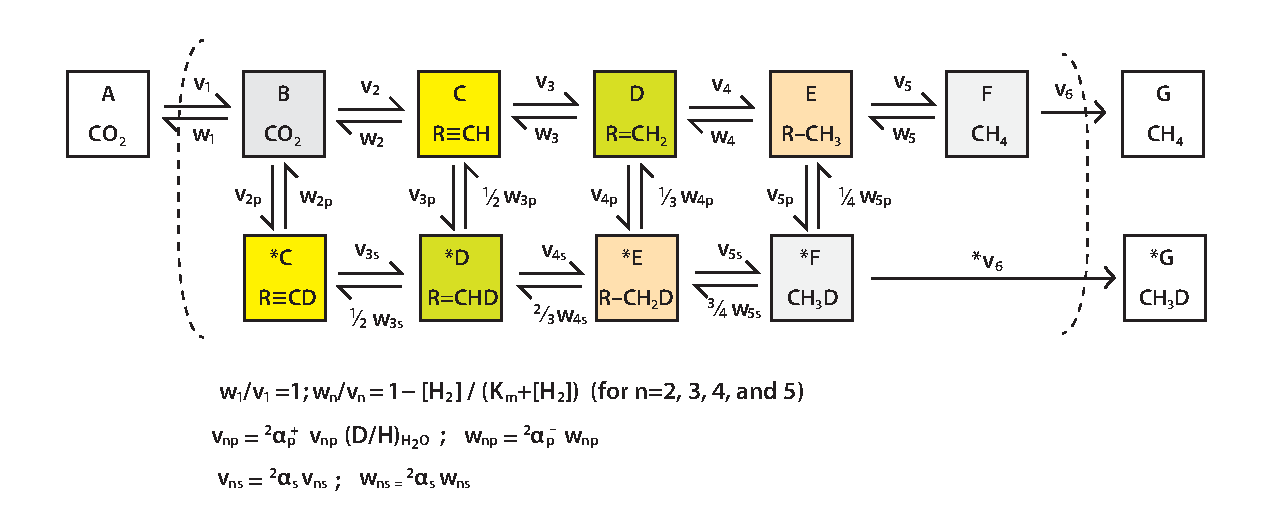
\includegraphics[width=0.9\linewidth]{figures/Fig2.S4}
	\caption[Schematic of the model of deuterium substitution during
	microbial methanogenesis from CO\textsubscript{2}]{Schematic of the model of deuterium substitution during
		microbial methanogenesis from CO\textsubscript{2}. Boxes represent
	pools of cellular carbon involved in the methanogenic pathway, and the
	asterisk represents a compound containing a deuterium substitution.
	Forward flows are represented by \emph{v}, and backwards flows are
	represented by \emph{w}. The model setup is similar in concept to
	previously published models for microbial sulfate reduction \parencite{Rees_1973_GCA,Brunner+Bernasconi_2005_GCA,Farquhar++_2007_GCA}.}
	\label{fig:2:S4}
\end{figure*}



\begin{SCfigure*}
	\centering
	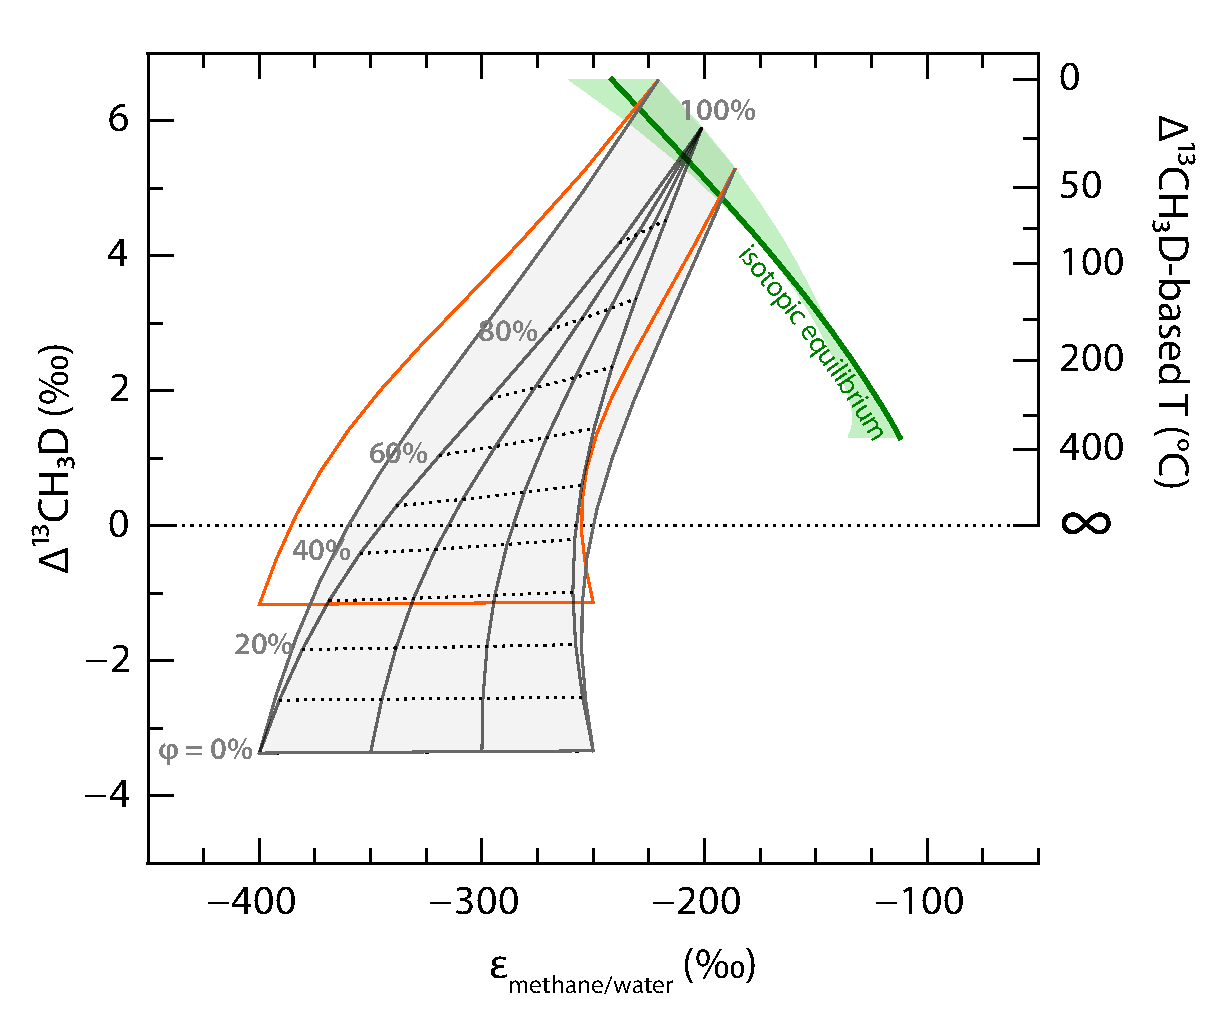
\includegraphics[width=0.5\linewidth]{figures/Fig2.S5}
	\caption[Dependence of model predictions on reversibility and fractionation
	factors]{Dependence of the modeled isotopic composition of microbial
		methane on the degree of reversibility and isotope fractionation
		factors. Orange and gray fields represent model output assuming a
		kinetic endmembers of $-$1.3‰ and $-$3.5‰, respectively (\autoref{tab:2:S3}). Inner
		solid gray lines represent model trajectories for 20~°C assuming
		different values for the D/H primary intrinsic isotope effect (\autoref{tab:2:S3}). Subhorizontal tie lines connect points of equal reversibility ($\varphi$).
		Outer solid lines represent bounding model trajectories calculated for 0
		and 40~°C.}
	\label{fig:2:S5}
\end{SCfigure*}

A mathematical model was constructed to describe isotopologue
compositions of methane produced from microbial methanogenesis (\autoref{fig:2:S4}). To allow for the use of data from studies on experimental and
natural systems as input parameters, our model simplifies the
representation of the biochemistry involved in the microbial generation
of methane, and only considers the production of methane via reduction
of CO\textsubscript{2}.

The model describes methanogenesis in six steps, and using an assumption
of steady-state intermediate compositions, solves for the abundances of
\textsuperscript{13}C- and D-substituted isotopologues of product
CH\textsubscript{4} and of four intermediate species (\autoref{fig:2:S4}). The
first step (1) is the uptake of CO\textsubscript{2} into the cell, and
the last step (6) is export of CH\textsubscript{4} out of the cell; we
assume that neither of these steps discriminates against isotopes or
between isotopologues. Inside the cell, the reduction of
CO\textsubscript{2} to CH\textsubscript{4} is treated in four steps
(steps \#2--5), where each step corresponds to the addition of one
hydrogen \parencite{Thauer_1998_M}.

The main variable input in our model is metabolic reversibility, which
is defined as the ratio of backwards to forwards fluxes
($\varphi_n = w_n \big/ v_n$) through an enzymatically-mediated reaction
sequence \parencite{Rees_1973_GCA,Hayes_2001_RiMG}. The reversibility is constrained by two
end-members, which represent fully-irreversible ($\varphi$ = 0; fully-kinetic)
and fully-reversible ($\varphi$ → 1; equilibrium) conditions. We parameterize the
reversibility as a simple function of H\textsubscript{2} concentration
by assuming Michaelis-Menten kinetics for each H-addition step:
\begin{equation}\label{eqn:phirevH2}
\varphi_n = 1 - \frac{[\ce{H2}]}{K_\text{M}+[\ce{H2}]}
\end{equation}
where \emph{n} represents the step number and \emph{K}\textsubscript{M}
is the effective half-saturation constant for H\textsubscript{2}
(assumed identical for steps 2--5). In our model, $\varphi$\textsubscript{1} is
set at 1 (i.e., CO\textsubscript{2} uptake is fully reversible).

Under an assumption of steady-state concentrations of intermediates, all
fluxes for the \textsuperscript{12}CH isotopologues are dependent upon
the methane formation rate (\emph{v}\textsubscript{6}, in e.g., mol
cell\textsuperscript{$-1$} s\textsuperscript{$-1$}) by:
\begin{equation}\label{eqn:methaneformationrate}
v_n=v_6/(1-\varphi_n ) \text{, and } w_n= \varphi_n v_6/(1-\varphi_n )
\end{equation}

A series of continuity equations can be written for each \textsuperscript{13}C-substituted isotopologue.  For example: 
%\begin{widetext}
\begin{equation}\label{eqn:continuityequations}
\frac{d^{13}\mathbf{D}}{dt} = {}_{\ }^{13}\alpha_{3}^{+} \cdot  v_{3} \cdot  {_{\ }^{13}r}_{\mathbf{C}} - \left(_{\ }^{13}\alpha_{4}^{+} \cdot v_{4} + {}_{\ }^{13}\alpha_{3}^{-} \cdot  w_{3} \right) \cdot  {_{\ }^{13}r}_{\mathbf{D}} + {}_{\ }^{13}\alpha_{4}^{-} \cdot  w_{4} \cdot {}_{\ }^{13}r_{\mathbf{E}}
\end{equation}
%\end{widetext}

Here, \textsuperscript{13}\textbf{D} is the abundance of
\textsuperscript{13}C-substituted isotopologues for the pool \textbf{D}
(i.e., R=CH\textsubscript{2}; \autoref{fig:2:S4}), and
\textsuperscript{13}\emph{r}\textbf{\textsubscript{X}} is the
isotopologue ratio of the pool \textbf{X} (where \textbf{X} =
\textbf{A}, \textbf{B}, \ldots{}, \textbf{F}), and
\textsuperscript{13}$\alpha$\emph{\textsubscript{n}}\textsuperscript{+} and
\textsuperscript{13}$\alpha$\emph{\textsubscript{n}}\textsuperscript{$-$} are the
\textsuperscript{13}C/\textsuperscript{12}C kinetic isotope effects
associated with the forward and backward reactions, respectively. There
are a total of five continuity equations for pools
\textsuperscript{13}\textbf{B}, \textsuperscript{13}\textbf{C},
\textsuperscript{13}\textbf{D}, \textsuperscript{13}\textbf{E}, and
\textsuperscript{13}\textbf{F}. Under an assumption of steady-state
concentrations of intermediate species (i.e.,
\emph{d}\textsuperscript{13}\textbf{X}/\emph{dt} = 0), we solve for the
ratios of \textsuperscript{13}C-containing to
\textsuperscript{12}C-containing isotopologues in the product methane
(\textbf{F}; i.e.,
\textsuperscript{13}CH\textsubscript{4}/\textsuperscript{12}CH\textsubscript{4})
and in the intermediates (\textbf{B}, \textbf{C}, \textbf{D}, and
\textbf{E}). The \textsuperscript{13}C/\textsuperscript{12}C ratio of
CO\textsubscript{2} (i.e., \emph{r}\textbf{\textsubscript{A}}) is
assigned.

For the deuterated isotopologues, the continuity equations account for
both primary isotope effects (describing the rates at which C--D bonds
are formed or broken relative to C--\textsuperscript{1}H bonds; fluxes
shown vertically in \autoref{fig:2:S4}) and secondary isotope effects (describing
the change in reaction rate resulting from D substitution at a site
\emph{adjacent} to that which is site of an
\textsuperscript{1}H-addition or abstraction reaction; fluxes shown
horizontally in \autoref{fig:2:S4}). For example for reservoir \textbf{D}, the continuity
equation for the D-substituted isotopologue (i.e., R=CH\textsubscript{2}
or R=CHD) is:
%\begin{widetext}
\begin{equation}\label{eqn:continuityeqnexampledeuterated}
\begin{split}
\frac{d^{2}\mathbf{D}}{{dt}} = {}_{\ }^{\ }{_{\ }^{2}\alpha_{3p}^{+} \cdot v_{3} \cdot {_{\ }^{2}r}_{\mathbf{H}} &+ {}_{\ }^{2}\alpha_{3s}^{+} \cdot v_{3} \cdot {_{\ }^{2}r}_{\mathbf{C}} \\
	&- \left( \tfrac{1}{2} \cdot {_{\ }^{2}\alpha}_{3s}^{-} \cdot w_{3} + \tfrac{1}{2} \cdot {}_{\ }^{2}\alpha_{3p}^{-} \cdot w_{3} + {}_{\ }^{2}\alpha_{4s}^{-} \cdot v_{4} \right) \cdot {_{\ }^{2}r}_{\mathbf{D}} \\&+ \tfrac{2}{3} \cdot {}_{\ }^{2}\alpha_{4s}^{-} \cdot w_{4} \cdot {_{\ }^{2}r_{\mathbf{E}}}_{\ }}
\end{split}
\end{equation}
%\end{widetext}

Here, \textsuperscript{2}$\alpha$\textsubscript{\emph{n}p} and
\textsuperscript{2}$\alpha$\textsubscript{\emph{n}s} are primary and secondary
deuterium isotope effects, 
\textsuperscript{2}\emph{r}\textsubscript{\textbf{X}} are D-isotopologue
ratios for reservoir \textbf{X}, and 
\textsuperscript{2}\emph{r}\textsubscript{\textbf{H}} is the D/H ratio of the
hydrogen source (i.e., cellular water). The stoichiometric factor
corresponds to the probability of a primary versus secondary
isotope-sensitive reaction occurring (in this case, there is a $\sfrac{2}{3}$ chance
of removing H from R--CH\textsubscript{2}D). Again, there are five linear
equations to be solved simultaneously. Conversion between isotopologue
ratios and isotope ratios requires consideration of reaction
stoichiometry. For example,
\begin{equation}
{}_{\ }^{2}r_\mathbf{D} = \frac{\left\lbrack \mathrm{R}{=}\mathrm{\text{CHD}} \right\rbrack}{\left\lbrack \mathrm{R}{=}\mathrm{C}\mathrm{H}_{\mathrm{2}} \right\rbrack} = 2\left( \frac{\mathrm{D}}{\mathrm{H}} \right)_{\mathrm{R}{=}\mathrm{C}\mathrm{H}_{\mathrm{2}}}\ 
\end{equation}

Clumped isotopologue ratios (e.g.,
{[}R=\textsuperscript{13}CHD{]}/{[}R=\textsuperscript{12}CH\textsubscript{2}{]})
can be solved for in a manner similar to that used for D-substituted
isotopologues above.

For simplicity, primary ($\alpha$\textsubscript{p}) and secondary
($\alpha$\textsubscript{s}) kinetic isotope fractionation factors for the four
H-addition steps are assumed to be identical at a given temperature
(fractionation factors calculated for a model temperature of 20~°C are
shown in \autoref{tab:2:S3}). The intrinsic (kinetic/forward)
\textsuperscript{13}C/\textsuperscript{12}C and D/H fractionation
factors are estimated from \emph{in vitro} and culture studies \parencite{Valentine++_2004_GCA,Hermes++_1984_Bc,Roston+Kohen_2010_PNAS,Scharschmidt++_1984_Bc,Scheller++_2013_JACS_KIE}. The intrinsic \textsuperscript{13}CD
fractionation factor ($\gamma$, where \textsuperscript{13D}$\alpha$ = $\gamma$ ·
\textsuperscript{13}$\alpha$ · \textsuperscript{2}$\alpha$) is taken to have the value
required to generate a Δ\textsuperscript{13}CH\textsubscript{3}D
signature of either $-$1.3‰ or $-$3.5‰ under fully-kinetic conditions (\nameref{main-text} and \autoref{tab:2:S3}). The \textsuperscript{13}C/\textsuperscript{12}C,
D/H, and \textsuperscript{13}CH\textsubscript{3}D equilibrium isotope
fractionation factors are based on experimental and/or theoretical
calibrations (\mrefs[]{Figs.}{fig:2:2}, \ref{fig:2:S1}, and \ref{fig:2:S3}) \parencite{Ono++_2014_AC,Horibe+Craig_1995_GCA,Cerrai++_1954,Horita_2001_GCA}. The intrinsic fractionation factors for the
reverse reactions ($\alpha$\textsuperscript{$-$}, \autoref{tab:2:S3}) are constrained by
the requirement for consistency among equilibrium ($\alpha$\textsubscript{eq}),
forward ($\alpha$\textsuperscript{+}), and reverse reactions (i.e.,
$\alpha$\textsubscript{eq} = $\alpha$\textsuperscript{$-$}/$\alpha$\textsuperscript{+}). We
note that varying the secondary isotope effect ($\alpha$\textsubscript{s},
assumed to be 0.84 in either direction, for all steps) changes the
curvature of the modeled microbial trajectories, but does not change the
endmember $\varepsilon$\textsubscript{methane/water} values (which are set by the
primary D/H isotope effect).

We initiated the model calculations at temperatures of 0, 20, and 40~°C.
These temperatures bracket the range of known or inferred environmental
temperatures at which the microbial methane samples we studied were
generated (\autoref{tab:2:S4}). The predicted isotopic compositions for microbial
methane generated between 0 and 40~°C are shown in \mrefs[]{Figs.}{fig:2:2} and \ref{fig:2:4}.

\begin{table}\centering
	
	\caption[Results of isotopic measurements of methane
	in samples of natural gas standards]{Results of isotopic measurements of methane
		in samples of natural gas standards NGS-1 and NGS-3. Uncertainties
		reported are 95\% confidence intervals over all measurement cycles for a
		single analysis as described in \autoref{spectroscopic-procedures}. Values for
		δ\textsuperscript{13}C, δD, and
		Δ\textsuperscript{13}CH\textsubscript{3}D are reported relative to PDB,
		SMOW, and the stochastic distribution, respectively.}
	\label{tab:2:S5}

	\begin{threeparttable}
		
		\begin{tabular}{l r@{\hspace{0.2em}}l r@{\hspace{0.2em}}l >{\raggedleft\arraybackslash}p{2.5em}@{\hspace{0.2em}}l r@{\hspace{0.2em}}l}
			% This notation >{\raggedleft\arraybackslash}p{5em} is for padding the left side so that multicolumn doesn't expand extra space on the right column of the multicolumn{2}{c}. http://stackoverflow.com/a/25690685
			\toprule
			Sample Name & \multicolumn{2}{c}{δ\textsuperscript{13}C (‰)} & \multicolumn{2}{c}{δD (‰)} &
			\multicolumn{2}{c}{Δ\textsuperscript{13}CH\textsubscript{3}D (‰)} & \multicolumn{2}{c}{\textit{T}\textsubscript{13D}
				(°C)}\tabularnewline
			\midrule
			NGS-1 & \textbf{$-$28.73} & ± 0.05  & \textbf{$-$137.47} & ± 0.05  &
			 \textbf{2.61} & ± 0.29  & \textbf{186} & +28/$-$24 \tabularnewline
			& \textbf{$-$28.79} & ± 0.07  & \textbf{$-$137.69} & ± 0.07  &
			\textbf{2.53} & ± 0.29  & \textbf{193} & +29/$-$25 \tabularnewline
			& \textbf{$-$28.91} & ± 0.05  & \textbf{$-$138.07} & ± 0.05  &
			\textbf{2.62} & ± 0.24  & \textbf{185} & +22/$-$19 \tabularnewline
			\midrule
			NGS-3 & \textbf{$-$72.82} & ± 0.06  & \textbf{$-$176.09} & ± 0.06  &
			\textbf{5.08} & ± 0.26  & \textbf{48} & +10/$-$9 \tabularnewline
			& \textbf{$-$72.71} & ± 0.05  & \textbf{$-$175.82} & ± 0.05  &
			\textbf{5.18} & ± 0.26  & \textbf{44} & +10/$-$9 \tabularnewline
			NGS-3 + 150ml air * & \textbf{$-$72.99} & ± 0.06  & \textbf{$-$176.21} & ±
			0.06  & \textbf{5.14} & ± 0.49  & \textbf{45} & +19/$-$17
			\tabularnewline
			\bottomrule
		\end{tabular}
	
		\begin{tablenotes}
			\item * This sample was a subsample of NGS-3 that was
			intentionally-contaminated with 150 ml of air, to check for artifacts
			introduced from sample preparation and analysis of samples containing
			large quantities of air. No significant difference was found compared to
			subsamples of NGS-3 that were not contaminated with air.	
		\end{tablenotes}
	
	\end{threeparttable}
\end{table}





\section{Supplementary Text}\label{supplementary-text}

\subsection{Evaluation of alternative mechanisms for isotopic
	disequilibria in microbial methane
}\label{evaluation-of-alternative-mechanisms-for-isotopic-disequilibria-in-microbial-methane}

There are several potential alternative mechanisms for the observed
isotopic disequilibria in microbial methane shown in \autoref{fig:2:2}. It is
conceivable that these signals are due to mixing of multiple methane
sources with differing δ\textsuperscript{13}C and δD values, as
Δ\textsuperscript{13}CH\textsubscript{3}D changes non-linearly upon
mixing. The magnitude of non-linearity in the mixing depends on the
difference in both δ\textsuperscript{13}C and δD values of the
endmembers. It can be shown, using a Taylor-series expansion
\parencite{Ono++_2006_GCA}, that two-component mixing of endmembers (A \& B) produces a
mixture with a Δ\textsuperscript{13}CH\textsubscript{3}D value of:
%\begin{widetext}
\begin{equation}\label{eqn:2:mixing}
\begin{split}
{{\Delta}^{{13}}\mathrm{\text{CH}}_{{3}}\mathrm{D}}_{\mathrm{\text{mixture}}} \approx {f}_{\mathrm{A}} \cdot {\Delta}^{{13}}\mathrm{\text{CH}}_{{3}}\mathrm{D}_{\mathrm{A}} &+ \left( {1 -}{f}_{\mathrm{A}} \right)\cdot{\Delta}^{{13}}\mathrm{\text{CH}}_{{3}}\mathrm{D}_{\mathrm{B}} \\
&+ {f}_{\mathrm{A}}\cdot\left( {1 -}{f}_{\mathrm{A}} \right)\cdot\left( {\updelta}^{{13}}\mathrm{C}_{\mathrm{A}}{-}{\updelta}^{{13}}\mathrm{C}_{\mathrm{B}} \right)\cdot\left( {\updelta}\mathrm{D}_{\mathrm{A}}{-}{\updelta}\mathrm{D}_{\mathrm{B}} \right)
\end{split}
\end{equation}
%\end{widetext}
where $f_\text{A}$ represents the fractional contribution
from endmember A. Accordingly, the observed \textasciitilde{}6‰ negative
bias in Δ\textsuperscript{13}CH\textsubscript{3}D values (from that
expected for equilibrium at 0--40~°C, \autoref{fig:2:1}) requires mixing of two
methane sources with δ\textsuperscript{13}C and δD values that differ by
±60‰ and $\mp$400‰, respectively; gases with these isotopic compositions are
unlikely to co-occur in the environments we studied \parencite{Whiticar_1990_OG}.

Alternatively, under a commonly-used classification based on
δ\textsuperscript{13}C and δD values \parencite{Whiticar_1999_CG}, methane from these
sites could be interpreted as derived from methyl-type fermentation
(\autoref{fig:2:1}). If so, the low Δ\textsuperscript{13}CD values could be
inherited from those of the C--H bonds in methyl groups of the organic
substrate(s). However, theoretical calculations predict consistent
Δ\textsuperscript{13}CD clumping effects of +6.2 ± 0.3‰ at 25~°C for the
C--H bond of simple organic compounds (\autoref{tab:2:S6}), which is not
significantly different from the equilibrium value for
Δ\textsuperscript{13}CH\textsubscript{3}D at 25~°C (+6.4‰). Thus,
inheritance of equilibrium Δ\textsuperscript{13}CD values from organic
precursors during methyl-type fermentation does not explain the observed
disequilibrium Δ\textsuperscript{13}CH\textsubscript{3}D signatures.
While inheritance of kinetically-influenced Δ\textsuperscript{13}CD
values from organic precursors is possible, the Δ\textsuperscript{13}CD
values of acetate and other methyl-bearing methanogenic substrates are
not currently known.

Furthermore, oxidation of methane can also be ruled out because the
substantial deuterium enrichment associated with methane oxidation
\parencite{Whiticar_1999_CG} is not observed in the samples we studied.

\begin{table}\centering
	
	\caption[Partition function ratios for
	simple organic compounds calculated at 25~°C]{Partition function ratios (\emph{β}-factors) for
		simple organic compounds calculated at 25~°C. Partition function ratios
	were calculated using the method of \textcite{Bigeleisen+Mayer_1947_JCP}.
	Vibrational frequencies were calculated using the Hartree-Fock method
	with the 6-31G* basis set. The partition function ratios listed below
	have been corrected with symmetry factors to account for changes in
	symmetry upon isotope substitution \parencite{Bigeleisen+Mayer_1947_JCP,Urey_1947_JChS}. The average
	Δ\textsuperscript{13}CD value calculated for methanol, formaldehyde,
	formate, methanethiol, and acetate is +6.2~±~0.3‰ (1\emph{s}).}
	\label{tab:2:S6}

	\begin{threeparttable}
		
		\begin{tabular}{ll cccc}
			\toprule
			Species & Formula* & \textsuperscript{13}C/\textsuperscript{12}C & D/H &
			\textsuperscript{13}CD/\textsuperscript{12}CH & Δ\textsuperscript{13}CD
			(‰)\tabularnewline
			\midrule
			Methane & C\textbf{H}\textsubscript{4} & 0.123 & 2.647 & 2.777 &
			6.4\tabularnewline
			Methanol & C\textbf{H}\textsubscript{3}OH & 0.150 & 2.812 & 2.968 &
			6.3\tabularnewline
			Formaldehyde & C\textbf{H}\textsubscript{2}O & 0.165 & 2.591 & 2.763 &
			6.7\tabularnewline
			Formate & \textbf{H}COOH & 0.200 & 2.834 & 3.040 & 5.9\tabularnewline
			Methanethiol & C\textbf{H}\textsubscript{3}SH & 0.128 & 2.759 & 2.893 &
			6.2\tabularnewline
			Acetate & C\textbf{H}\textsubscript{3}COOH & 0.147 & 2.775 & 2.927 &
			6.0\tabularnewline
			\bottomrule
		\end{tabular}
	
		\begin{tablenotes}
			\item * D/H and \textsuperscript{13}CD/\textsuperscript{12}CH \emph{β}-factors
			were calculated for D substitution at H sites shown in bold letters.
		\end{tablenotes}
	
	\end{threeparttable}

\end{table}

\subsection{The equilibrium hydrogen-isotopic fractionation between
	water and methane
}\label{the-equilibrium-hydrogen-isotopic-fractionation-between-water-and-methane}

We compiled previously-published equilibrium hydrogen-isotopic
fractionation factors calibrated at various temperatures, either
experimentally or theoretically, for the system
CH\textsubscript{4}(\emph{g})-H\textsubscript{2}(\emph{g})-H\textsubscript{2}O(\emph{g})-H\textsubscript{2}O(\emph{l}).
The H\textsubscript{2}O(\emph{l})/H\textsubscript{2}(\emph{g})
fractionation factor is very large ($\alpha$ is \textasciitilde{}4 at room
temperature), and calibrations diverge substantially at lower
temperatures (\textless{}100~°C, \autoref{fig:2:S3}); this is the main source of
uncertainty in estimates of
CH\textsubscript{4}(\emph{g})/H\textsubscript{2}O(\emph{l}) equilibrium
D/H fractionation, which is derived by combination of
H\textsubscript{2}O(\emph{l})/H\textsubscript{2}(\emph{g}),
H\textsubscript{2}(\emph{g})/H\textsubscript{2}O(\emph{g}), and
CH\textsubscript{4}(\emph{g})/H\textsubscript{2}(\emph{g}) calibration
curves. We used the \textcite{Cerrai++_1954} calibration for
H\textsubscript{2}O(\emph{l})\slash H\textsubscript{2}(\emph{g}) in the
calculation of $\varepsilon$\textsubscript{methane/water} of the equilibrium
endmember of our model for isotope effects accompanying microbial
methanogenesis (see \autoref{model-of-isotopologue-systematics-during-microbial-methanogenesis}) because amongst the published
calibrations, this is likely most accurate at lower temperatures \parencite{Horibe+Craig_1995_GCA,Roston+Kohen_2010_PNAS,Suess_1949}. The uncertainty in calibration, as
well as salt and pressure effects \parencite{Horita_2005_GcJ}, could explain small
apparent offsets from the equilibrium line (\autoref{fig:2:2}) for some samples of
thermogenic methane.

\subsection{Field site descriptions and sampling
	methods}\label{field-site-descriptions-and-sampling-methods}

\emph{Bovine rumen, State College, Pennsylvania, USA.} The bovine rumen
gas samples obtained for this study were collected from cannulated,
lactating Holstein dairy cows at The Pennsylvania State University using
methods described previously \parencite{Tekippe++_2011_JoDS}. The samples were stored at
room temperature in glass serum vials stoppered with blue butyl septa.
Bovine rumen fluid was also sampled for water isotope analysis (\autoref{tab:2:S4}). The fluid was centrifuged to remove large particulate material,
filtered with a 0.2~µm filter, and distilled to remove dissolved organic
matter prior to isotope-ratio analysis. We note that the rumen fluid and
gas samples were not taken from the same animal at the same time.
However, the temporal variation of δD of tap water in the U.S. is
expected to be small (generally \textless{}10‰ in any particular region
over multiple seasons) \parencite{Bowen++_2007_WRR}.

\emph{Northern Cascadia Margin.} Gas samples were collected from gas
voids and hydrates in sediment cores drilled during IODP (Integrated
Ocean Drilling Program) Expedition 311 \parencite{IODP_x311_Proceedings}. These gases were
interpreted to be dominantly microbial based on isotopic and
compositional analyses (e.g., C\textsubscript{1}/C\textsubscript{2}
\textgreater{} 1000) \parencite{Pohlman++_2009_EPSL}. The gas samples were subsampled for
previous analyses, and have remained in archive since. Samples were
contained either in serum vials sealed with blue butyl stoppers, or in
Vacutainers® (Becton Dickinson) sealed with orange septa and an
additional silicone plug (in \autoref{tab:2:S1}, these are denoted ``SB'' or
``Vac'', respectively); these methods are standard IODP procedures. The
sample ID's for the samples from the Northern Cascadia Margin listed in
\autoref{tab:2:S1} are the same as those reported in \textcite{Pohlman++_2009_EPSL}.

\emph{Powder River Basin, Montana, USA.} The Powder River Basin is a
major source of coal and coalbed methane. Gas samples were collected
from multiple gas wells producing from the methane-rich Wall and Canyon
coal seams using a wellhead gas sampler and IsoTubes (from Isotech
Laboratories, Champaign, Illinois, USA). Water samples were collected
concurrently from the same wells, filtered through 0.45~µm nylon
filters, transported to the lab on ice in deionized water-washed glass
bottles with no headspace, and kept at 4 \textsuperscript{o}C prior to
analysis.

\emph{Atlantic White Cedar swamp, Cape Cod, Massachusetts, USA.}
Atlantic White Cedar swamps are wetlands found throughout the coastal
northeastern United States \parencite{Laderman++_1989}. We collected gases and water
from a swamp (``Swamp Y'', approximate coordinates \ang[minimum-integer-digits=2]{41;31;38.2}N,
\ang[minimum-integer-digits=2]{70;39;15.5}W) on the campus of the Marine Biological Lab (MBL) in Woods
Hole, MA in May 2014. Gases were collected by trapping the bubbles
released when sediment on the bottom of the swamp was gently disturbed.
The collected gases were transferred via syringes to serum vials (either
pre-evacuated or pre-filled with NaCl brine that was displaced to make
room for the gas sample) sealed with blue butyl septa, and stored at
room temperature until analysis. One sample (``SwampY-5'', \autoref{tab:2:S1}) was
subsampled and analyzed 3 days after sample collection, and again 3
weeks later. The measured Δ\textsuperscript{13}CH\textsubscript{3}D
values were indistinguishable within the precision of the measurements
(0.36 ± 0.34‰ and 0.27 ± 0.52‰, respectively).

\emph{Upper Mystic Lake, Arlington, Massachusetts, USA.} Upper Mystic
Lake is a freshwater lake in the Boston metropolitan area. Ebullition of
methane from this lake has been previously documented \parencite{Varadharajan+Hemond_2012_JGR,Scandella++_2011_GRL}. We collected gas bubbles using inverted funnel-shaped bubble
traps {[}modified from an inverted-funnel design described previously
\parencite{Varadharajan+Hemond_2012_JGR,Varadharajan++_2010_LOM}{]} deployed \textasciitilde{}2 m above the lake
floor (\textasciitilde{}18 m water depth) using a custom rope and buoy
structure.\footnote{A description of the apparatus appears in \textcite{Delwiche++_2015_LOM}.} The deep deployment depth was chosen to minimize dissolution
and/or oxidation of bubbles during their transit from the sediment to
the lake surface. The collected gases were transferred via syringes to
serum vials (either pre-evacuated or pre-filled with deionized water
that was displaced to make room for the gas sample) sealed with blue
butyl septa, fixed with either saturated NaCl solution or 1~M NaOH, and
stored at either 4~°C or room temperature until analysis. The water
sample from Upper Mystic Lake listed in \autoref{tab:2:S4} was collected in
September 2014.

\emph{Lower Mystic Lake, Arlington, Massachusetts, USA.} Lower Mystic
Lake (elevation 1 m above sea level, maximum depth 24~m) is a meromictic
glacial kettle lake. The sample of methane reported in \autoref{tab:2:S1} was
extracted from water we collected from 20~m water depth (mbll, meters
below lake level) in August 2014. The water sample was transferred into
a 2~L media bottle, taking care to minimize bubbles, immediately
stoppered with a black rubber septum (Glasgerätebau Ochs, Germany), and
transported to the laboratory. A headspace was created using helium, and
the sample was then stored at 4~°C until extraction and analysis. The
concentration of dissolved methane at 20 mbll was determined to be
4.2~mM (±5\%). Field measurements indicated that the water at 20 mbll
was oxygen-depleted and had elevated conductivity relative to surface
water. The water sample listed in \autoref{tab:2:S4} was collected from 18 mbll,
which is below the chemocline.

\emph{The Cedars, Cazadero, California, USA.} Samples of bubbling gases
were collected in June 2013 and July 2014 from sites in The Cedars as
described in \textcite{Morrill++_2013_GCA}; the sites studied here were
Barnes Spring Complex (BSC), and Nipple Spring (NS). Gas samples were
collected in inverted-bucket traps positioned over seeps, and collected
gases were transferred to serum bottles stoppered with blue butyl rubber
septa. Samples were fixed with HgCl\textsubscript{2} or HCl to prevent
microbial alteration of the methane.

\emph{Coast Range Ophiolite Microbial Observatory, Lower Lake,
	California, USA.} The Coast Range Ophiolite Microbial Observatory,
located at the McLaughlin Natural Reserve (UC Davis), was established in
2011 with the completion of eight ultramafic-hosted groundwater
monitoring wells drilled using a mud-free technique \parencite{Cardace++_2013_SD,Crespo-Medina++_2014_FMicro}. Water was sampled from well ``N-08A'' in December 2013 using
a bladder pump into 1--2 L bottles, stoppered immediately as described
above for the Lower Mystic Lake sample, transported to the laboratory,
and stored at 4~°C until extraction and analysis. We also collected
water in July 2014 from an electrically-pumped non-potable groundwater
well in the Core Shed area (``CSWold'', approximate coordinates
\ang[minimum-integer-digits=2]{38;51;42.53}N, \ang[minimum-integer-digits=2]{122;24;53.05}W). For this sample, dissolved gases were
extracted on-site via equilibration with a helium headspace and stored
in a stoppered serum vial fixed with 0.5~ml 1~M HCl. The water sample
for which the δD\textsubscript{water} value is reported in \autoref{tab:2:S4} was
collected from CSWold in December 2013. The range of H\textsubscript{2}
concentrations reported in \autoref{tab:2:S4} from CROMO are minimum and maximum
values of {[}H\textsubscript{2}{]} observed over multiple sampling trips
during a long-term (\textasciitilde{}3 years) sampling campaign.

\emph{Kidd Creek Mine, Timmins, Ontario, Canada.} In subsurface mines in
the Canadian Shield, exploration boreholes intersecting extensive
fracture networks release waters rich in reduced gases
(H\textsubscript{2}, CH\textsubscript{4}, C\textsubscript{2+}) and noble
gases, which exsolve upon depressurization. Sampling and
characterization of fracture fluids from Kidd Creek have been described
in previous studies \parencite{SherwoodLollar++_2008_GCA,SherwoodLollar++_2002_N,Holland++_2013_N,SherwoodLollar++_2007_Ab,Sherwood++_1988_CG}. We analyzed methane sampled from boreholes at the 7850$'$- and
9500$'$-levels (\autoref{tab:2:S1}). These samples were taken between 2007 and 2014,
and stored in glass serum vials stoppered with blue butyl rubber septa.
The δ\textsuperscript{13}C values of these gases were previously
measured by GC-IRMS at the University of Toronto. No evidence of any
effects of long-term storage on the δ\textsuperscript{13}C of methane in
these samples has been observed; the average difference between
δ\textsuperscript{13}C determined via TILDAS compared to GC-IRMS was
0.09 ± 0.60‰ (1\emph{s}, \emph{n} = 9), and shows no correlation with
the length of time the sample had been stored.

\emph{Guaymas Basin hydrothermal system (Rebecca's Roost vent), Gulf of
	California.} Guaymas Basin in the Gulf of California hosts an active
sediment-hosted mid-ocean ridge hydrothermal
system \parencite{Didyk+Simoneit_1989_N,Simoneit_1985_CJES,Simoneit_Lonsdale_1982_N}. We analyzed methane from a sample
of a 299~°C vent fluid emanating from Rebecca's Roost, a
flange-like vent structure. The sample was taken in 2008 using a
isobaric gas-tight sampler (\autoref{tab:2:S1}) and poisoned with mercuric
chloride \parencite{Seewald++_2002_DSR}. Fluid properties and geochemical data associated
with this sample have been previously published \parencite{Reeves++_2014_PNAS}. We assumed
a value of +4 ± 2‰ for the δD\textsubscript{water} of the vent fluid
based on previous observations of Guaymas Basin hydrothermal fluids \parencite{Shanks++_1995_AGU-GM}.

\emph{Northern Appalachian Basin, Central Pennsylvania, USA.} Gases were
sampled from gas wells producing from the Marcellus Formation (Middle
Devonian) and Utica Formation (Upper Ordovician) in central Pennsylvania
using standard wellhead sampling techniques. Gases produced from these
geologic units are dry (\textless{}5\%
C\textsubscript{2+}/$\big\sum\!$C\textsubscript{1--5}) thermogenic gases of high
thermal maturity \parencite{Baldassare++_2014_AAPGB,Stolper++_2014_S}. The
C\textsubscript{1}/C\textsubscript{2} ratios of the gas samples from the
Marcellus and Utica Shales we analyzed were \textless{}100 (\autoref{tab:2:S4}),
which is within the range expected for thermogenic gases \parencite{Bernard++_1978_JGR,Bernard++_1976_EPSL}.





